\documentclass{beamer}
\usepackage{animate}
\usepackage{graphicx}
\usepackage{pgffor} 
\usepackage[T1]{fontenc}
\usepackage{amsmath}
\usepackage[utf8]{inputenc}
\usepackage[german]{babel}
\usepackage[scaled]{helvet}
\renewcommand{\familydefault}{\sfdefault}
\usepackage{blindtext}
\usepackage{adjustbox}
\usepackage{calc}
\usepackage{listings}
\usepackage{xcolor}
\usepackage{geometry}
\usepackage{longtable}
\usepackage{array}
\usepackage{tabularx}
\usepackage{hyperref,graphicx}   
\usepackage{caption}
\usepackage{refstyle}
\usepackage{pdfpages}
\usepackage{comment}
\usepackage{listings}
%\usepackage{xcolor}
%\graphicspath{{bilder/}}
\usepackage{import}
%\usepackage[dvipsnames,table]{xcolor}
%\usepackage{hyperref}
%\us^epackage{multirow}
%\usepackage{textpos}
\usepackage{color}
\usepackage{tikz}
\usepackage{pgfplots}
\usepackage{ragged2e}
\usepackage{blindtext}

\lstset{
    language=Python,
    backgroundcolor=\color{white},   % Choose the background color
    basicstyle=\ttfamily\footnotesize, % Choose the font and size
    keywordstyle=\color{blue},        % Color for keywords
    commentstyle=\color{green},       % Color for comments
    stringstyle=\color{red},          % Color for strings
    numbers=left,                    % Line numbers on the left
    numberstyle=\tiny\color{gray},    % Style for line numbers
    stepnumber=1,                    % Line number step
    numbersep=5pt,                   % Distance between line numbers and code
    showstringspaces=false,          % Don't underline spaces in strings
    breaklines=true                  % Allow line breaks if code exceeds width
}
\hypersetup{
    colorlinks=magenta,
    linkcolor=blue,
    filecolor=magenta,      
    urlcolor=cyan,
    pdftitle={Overleaf Example},
    pdfpagemode=FullScreen,
    }

\usetheme{Berlin}
\setbeamercolor{item}{fg=cyan} % Change item color
%\setbeamercolor{section in toc}{fg=cyan} % Change section color in table of contents
\setbeamercolor{alerted text}{fg=cyan} % Change alert text color
\setbeamercolor{block title}{bg=blue, fg=white} % Change block title color
\setbeamercolor{block body}{bg=lightgray, fg=black} % Change block body color
\definecolor{myblue}{RGB}{0, 102, 104} 

\title{Rekursion}

\titlegraphic{
\includegraphics[scale=0.2]{bilder/hsh.png}}
\author{Thanh Viet Nguyen, Fourat Zai El Amri, Luis Sperling,
Daniel Pessler, Mikhail Safonov} 
\institute[]{Hochschule Hannover}
\date{15.11.2024}


\begin{document}

\logo{}
\begin{frame}
    \titlepage 
\end{frame}

%\logo{
\includegraphics[scale=0.1]{bilder/hsh.png}}

\begin{frame}{Agenda}
    \tableofcontents
\end{frame}


\section{Einleitung}
\begin{frame}{Einleitung}
\begin{itemize}
    \item Was ist Rekursion?
    \item Wozu ist sie da?
\end{itemize}
\end{frame}
\begin{frame}
    \begin{center}
           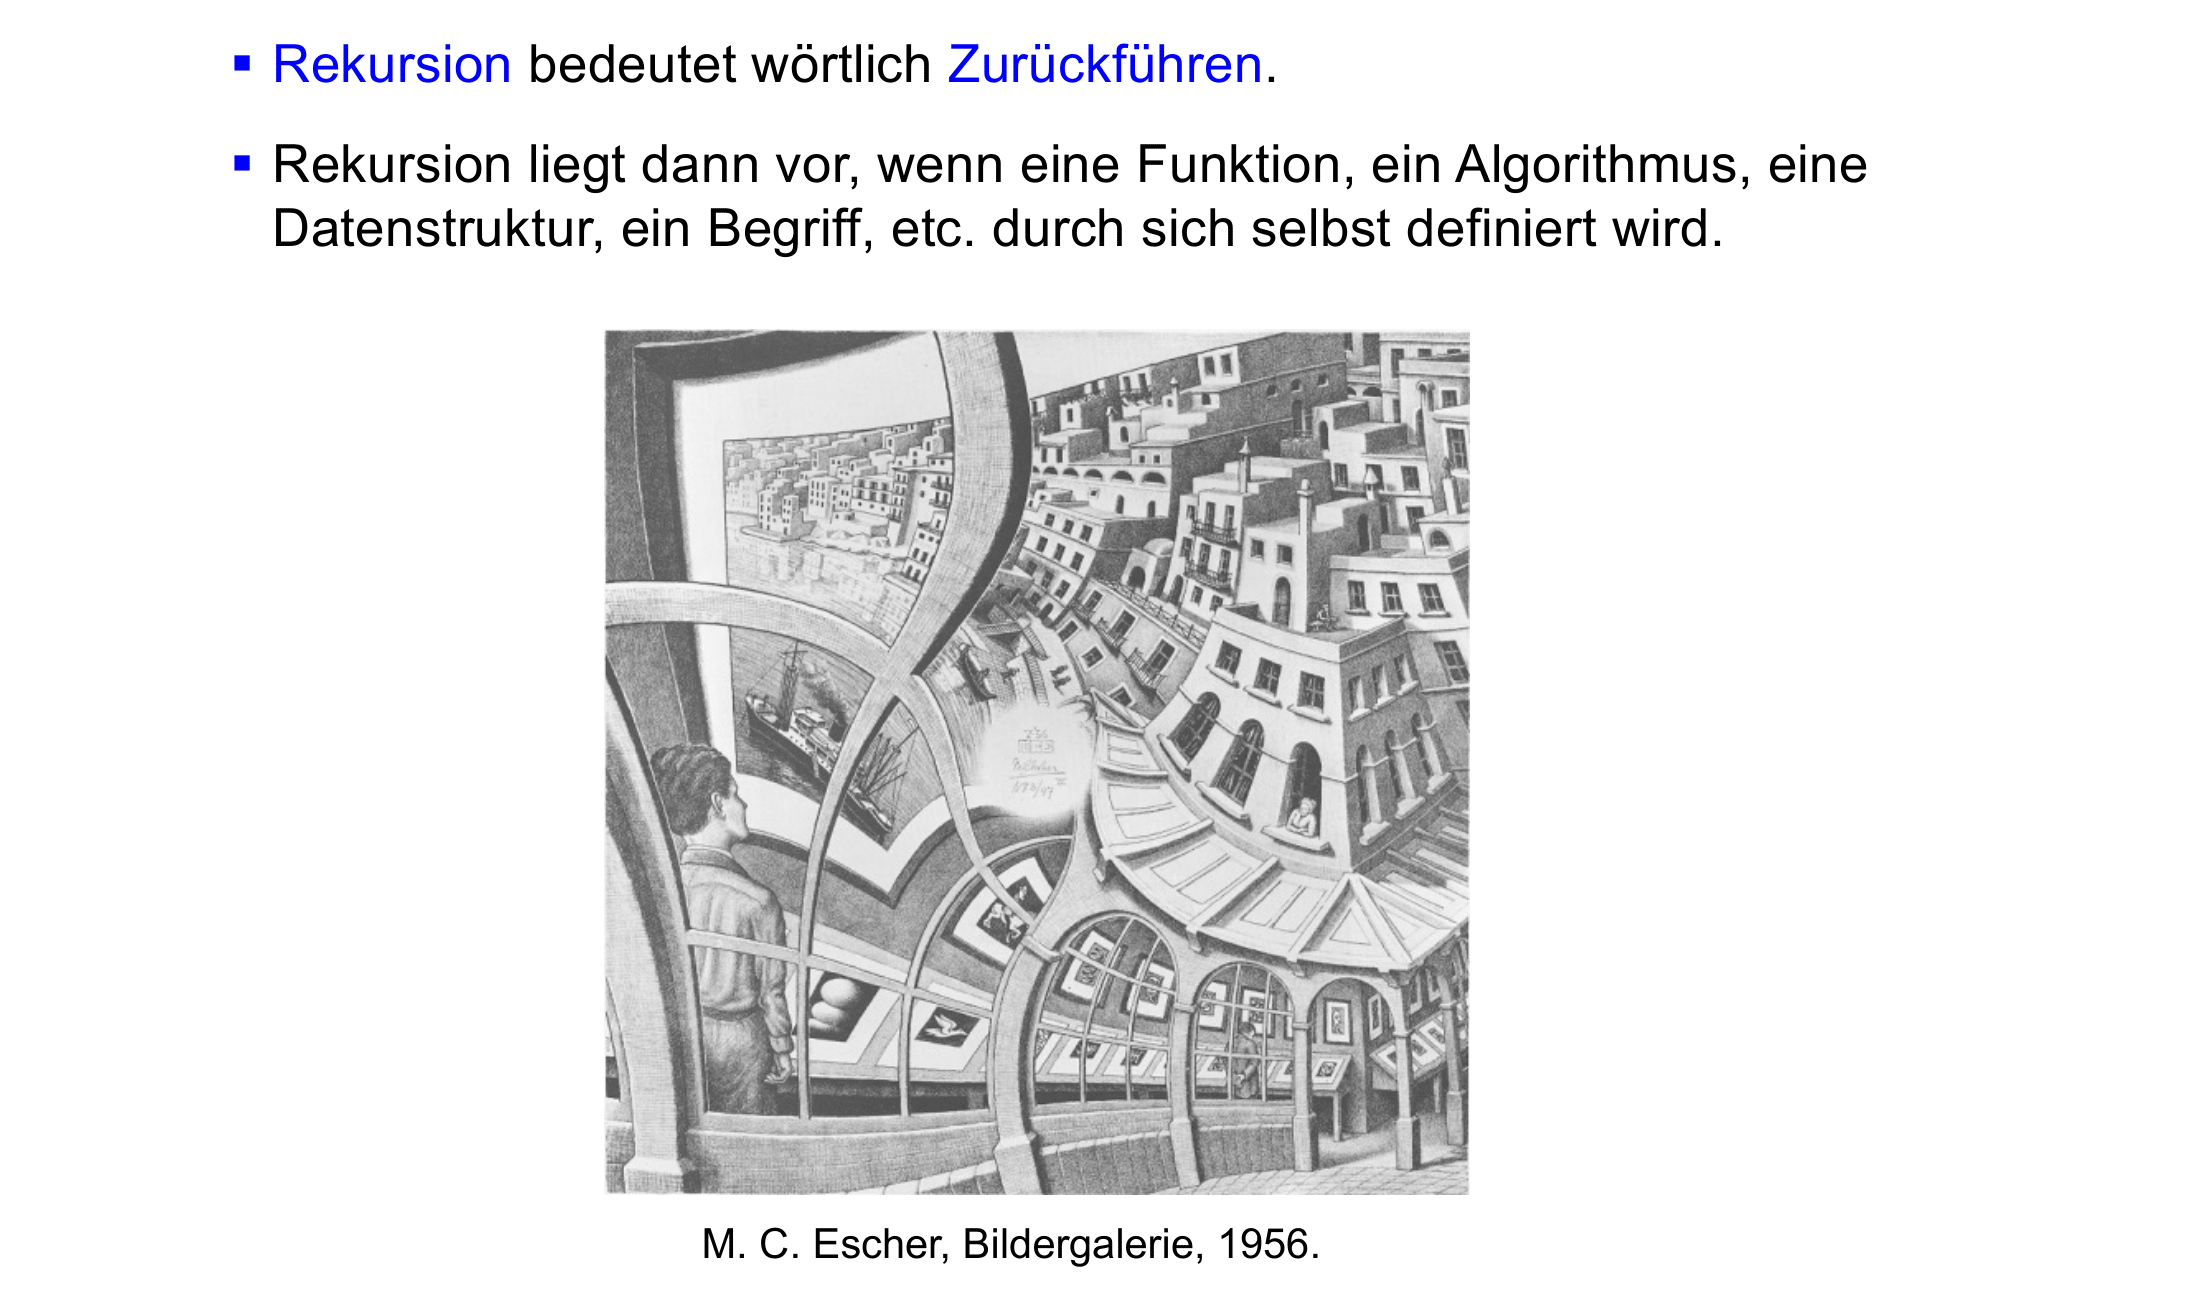
\includegraphics[width=1.1\textwidth]{rekursion anlage/07_Rekursion-02.png}
    \end{center}
\end{frame}
\begin{frame}
    \begin{center}
           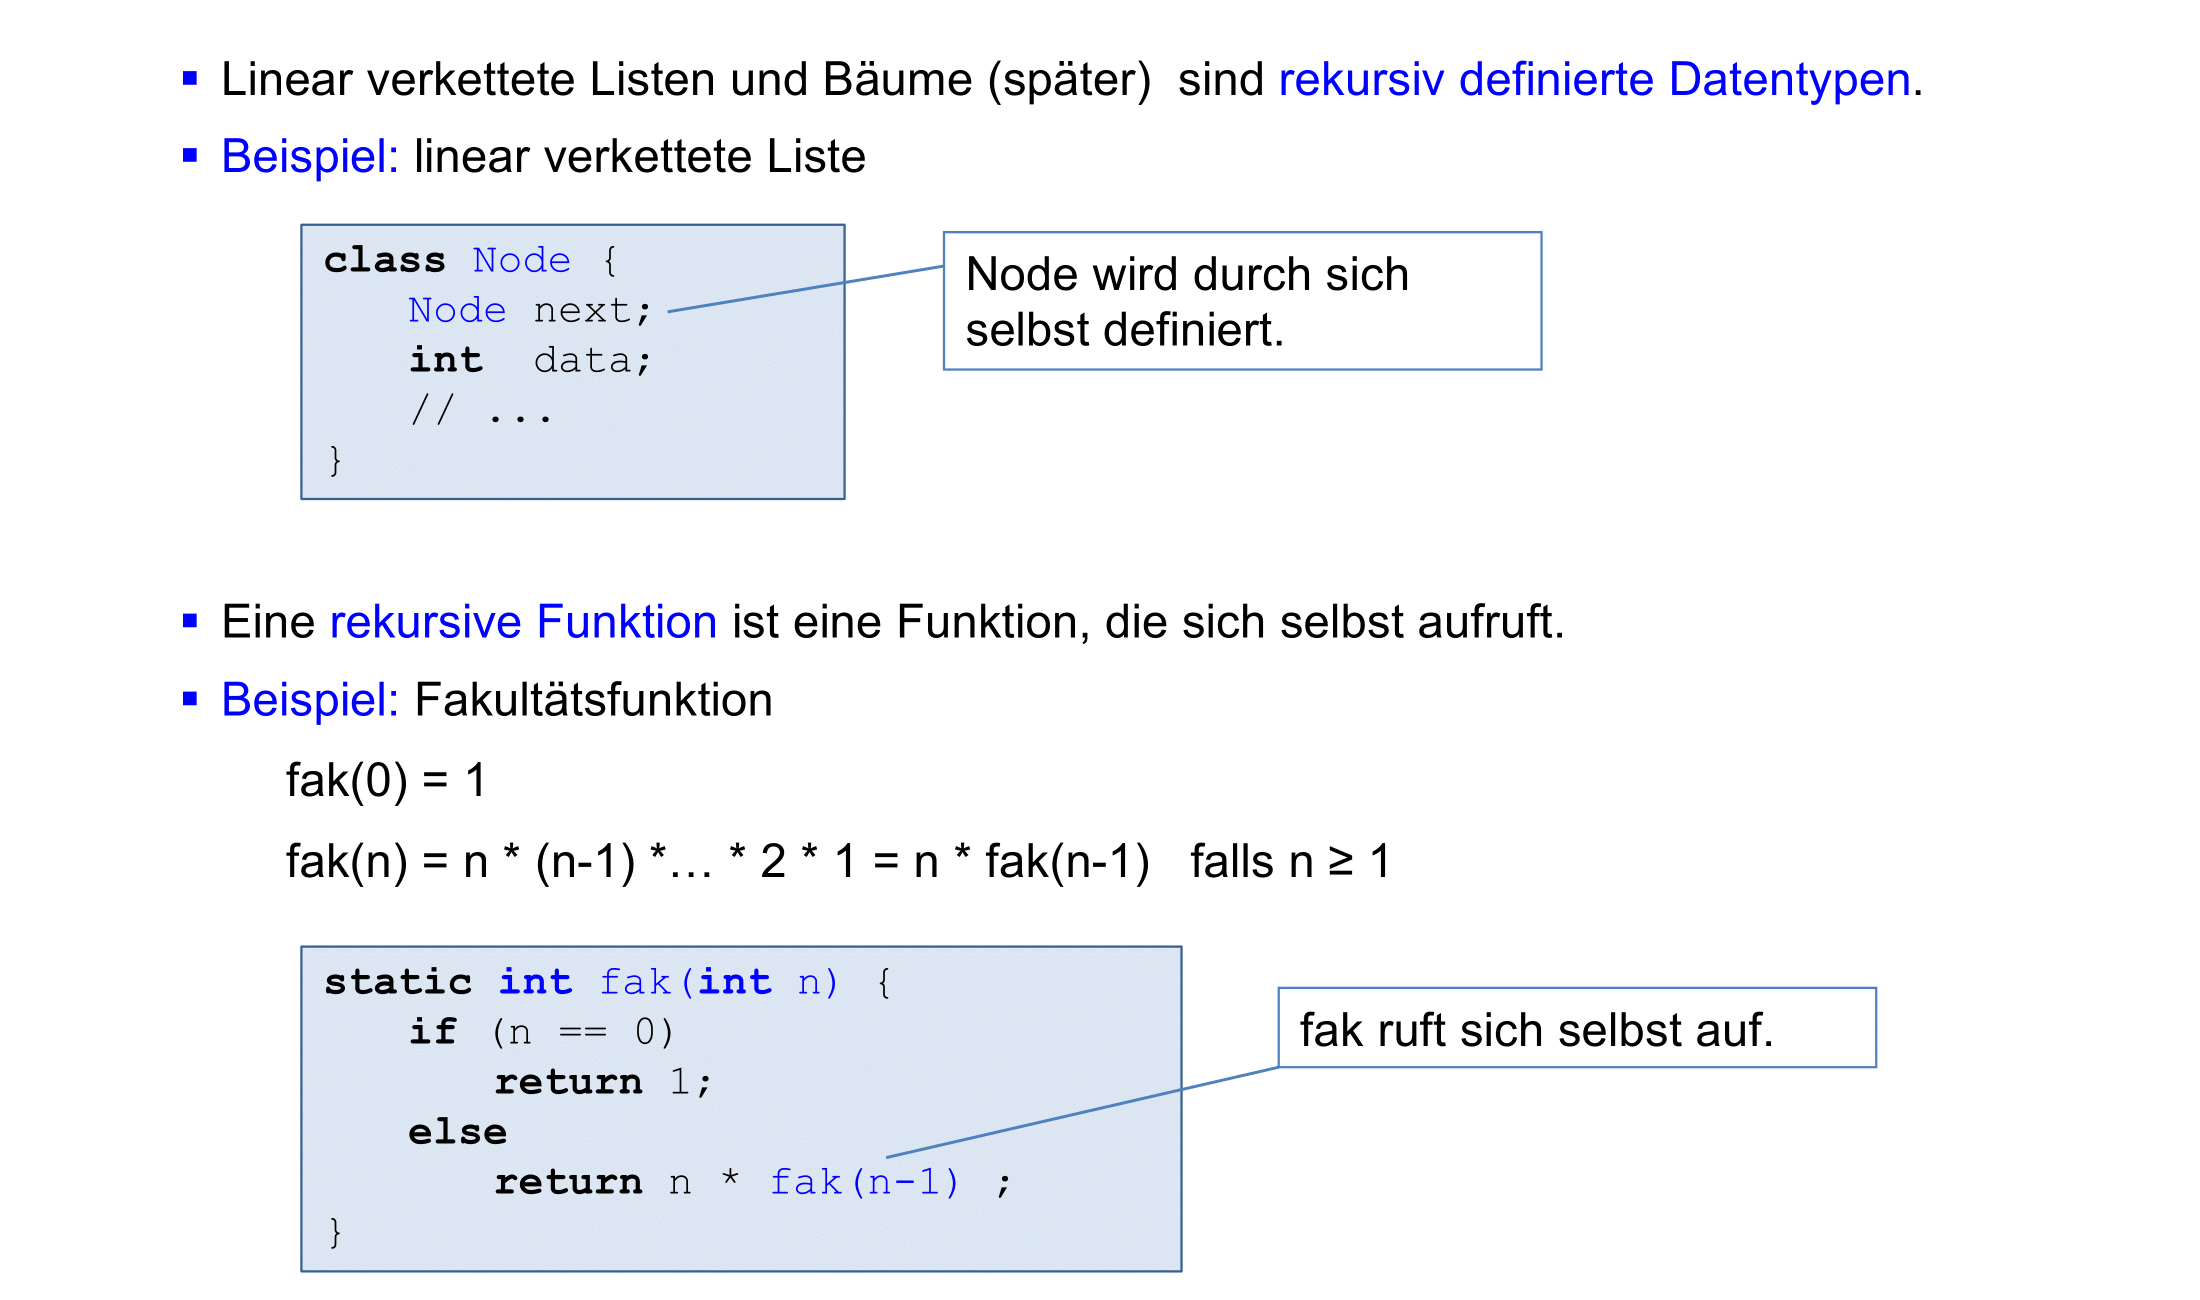
\includegraphics[width=1.1\textwidth]{rekursion anlage/07_Rekursion-03.png}
    \end{center}
\end{frame}
\begin{frame}
    \begin{center}
           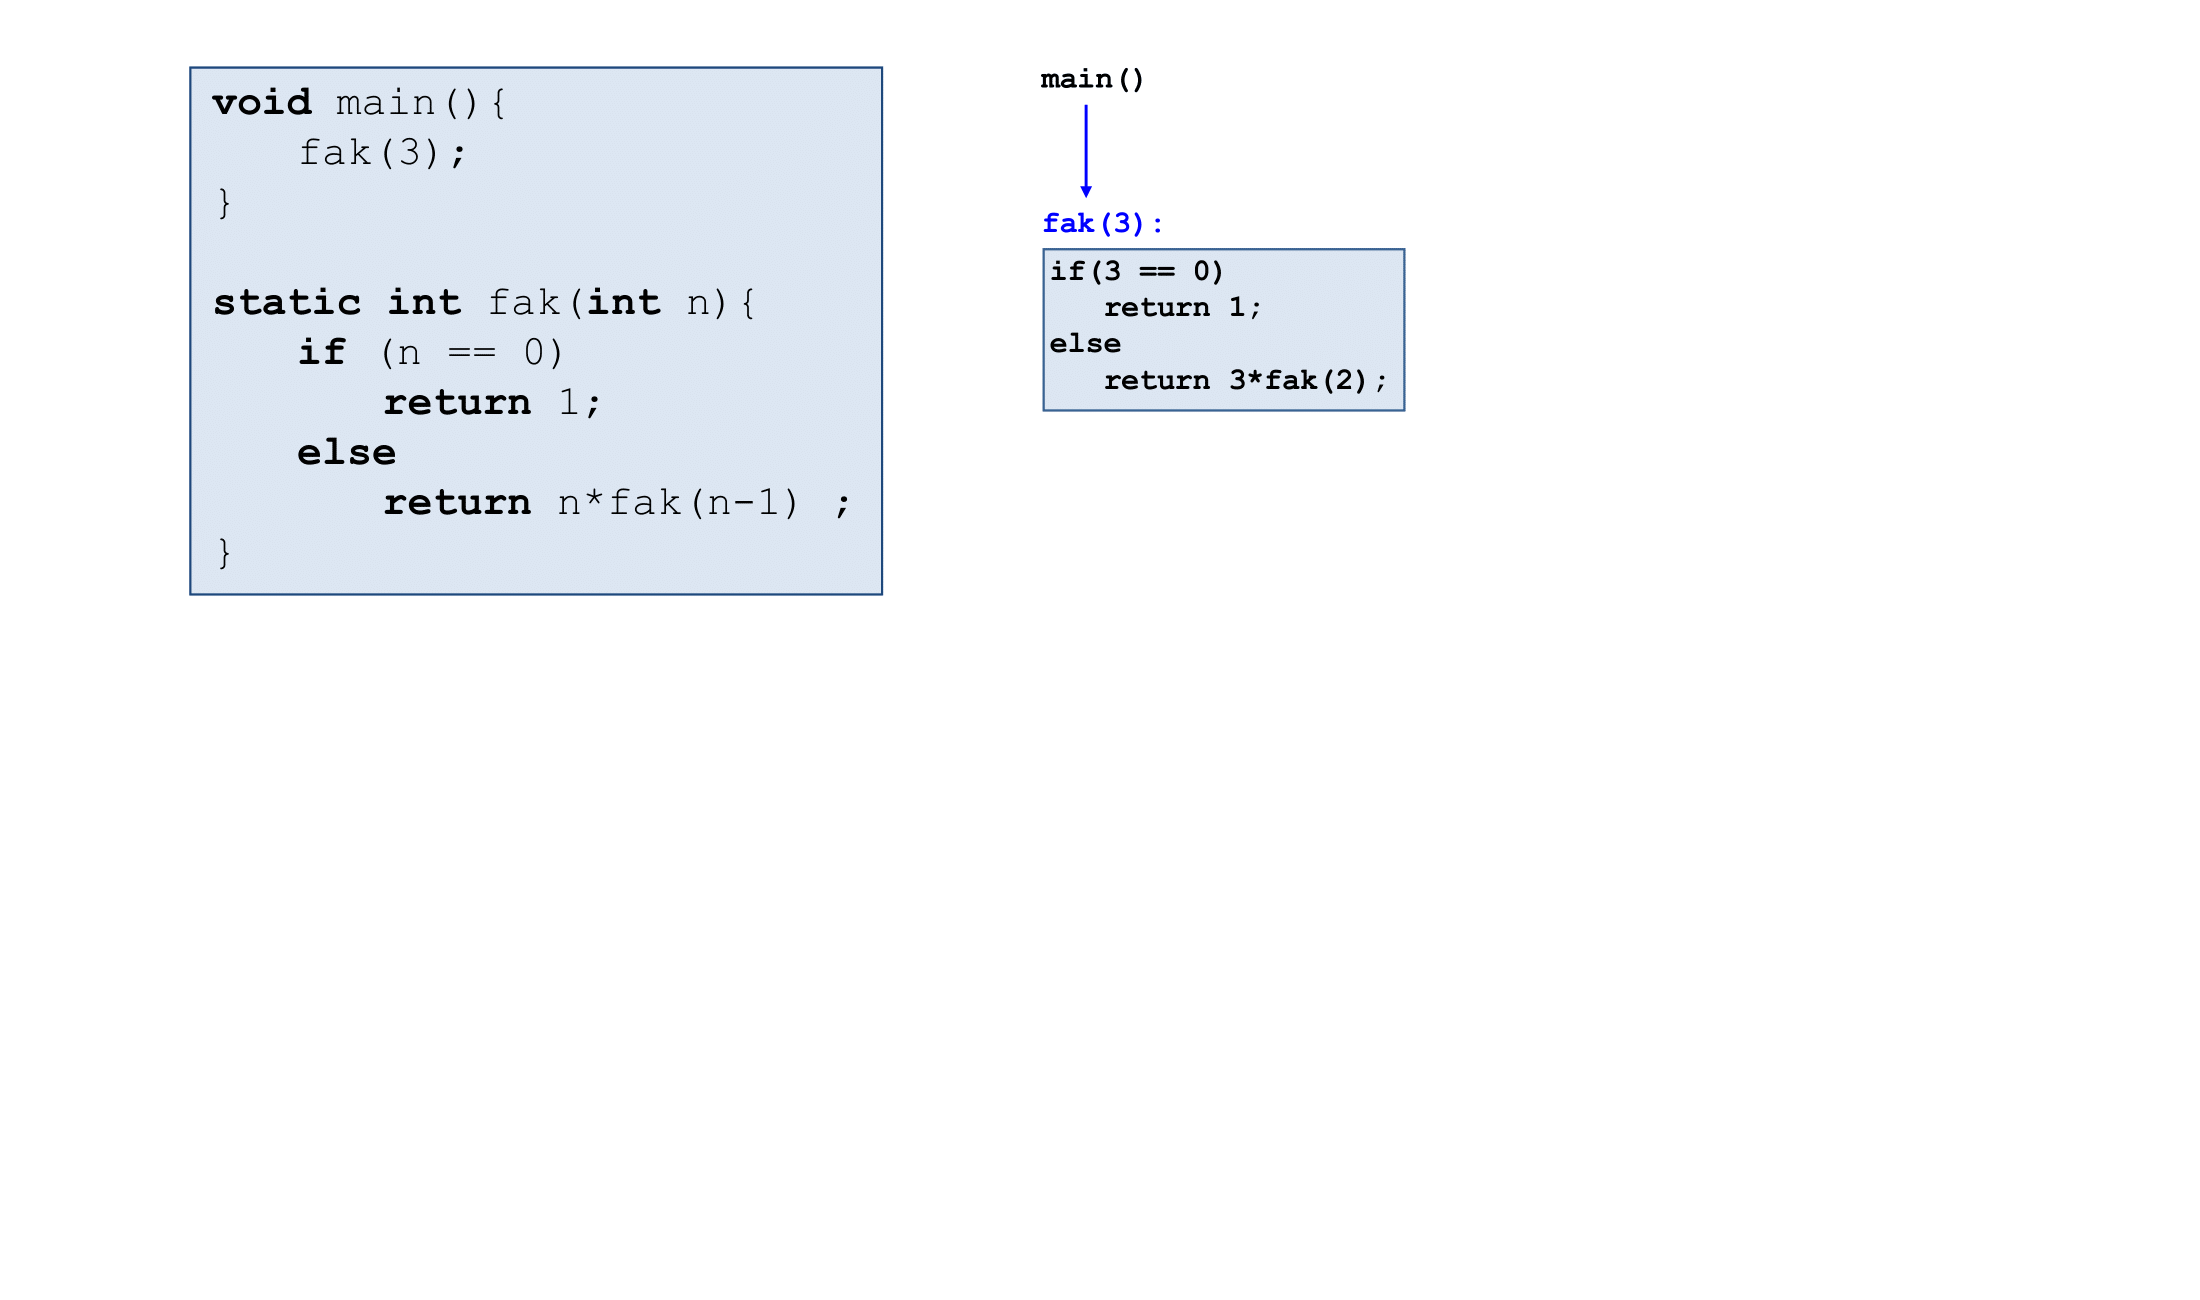
\includegraphics[width=1.1\textwidth]{rekursion anlage/07_Rekursion-04.png}
    \end{center}
\end{frame}
\begin{frame}
    \begin{center}
           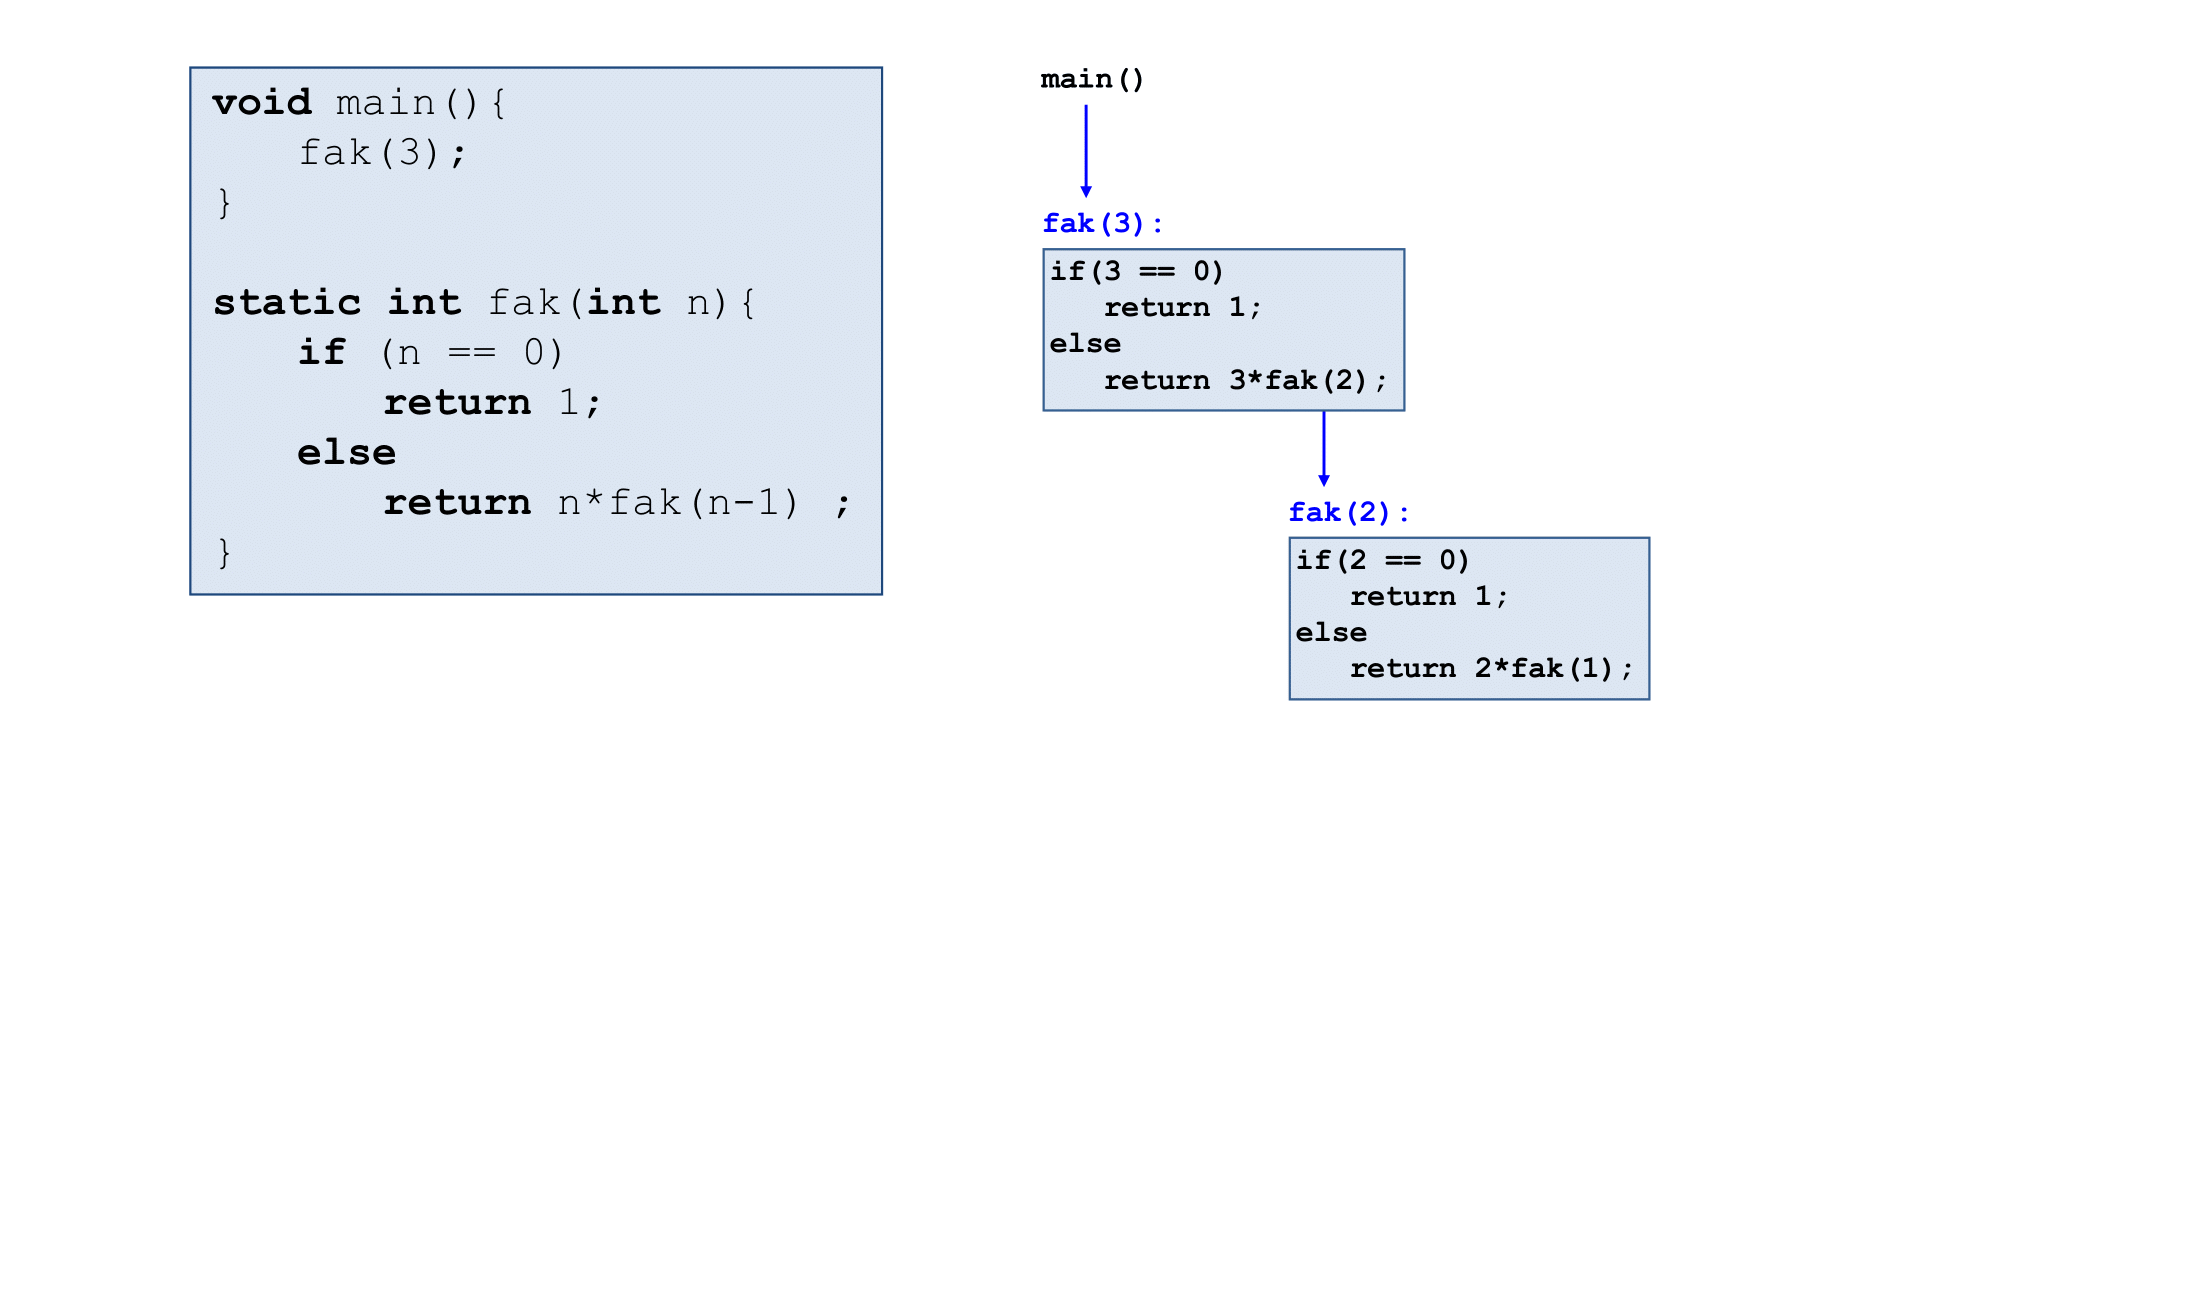
\includegraphics[width=1.1\textwidth]{rekursion anlage/07_Rekursion-05.png}
    \end{center}
\end{frame}
\begin{frame}
    \begin{center}
           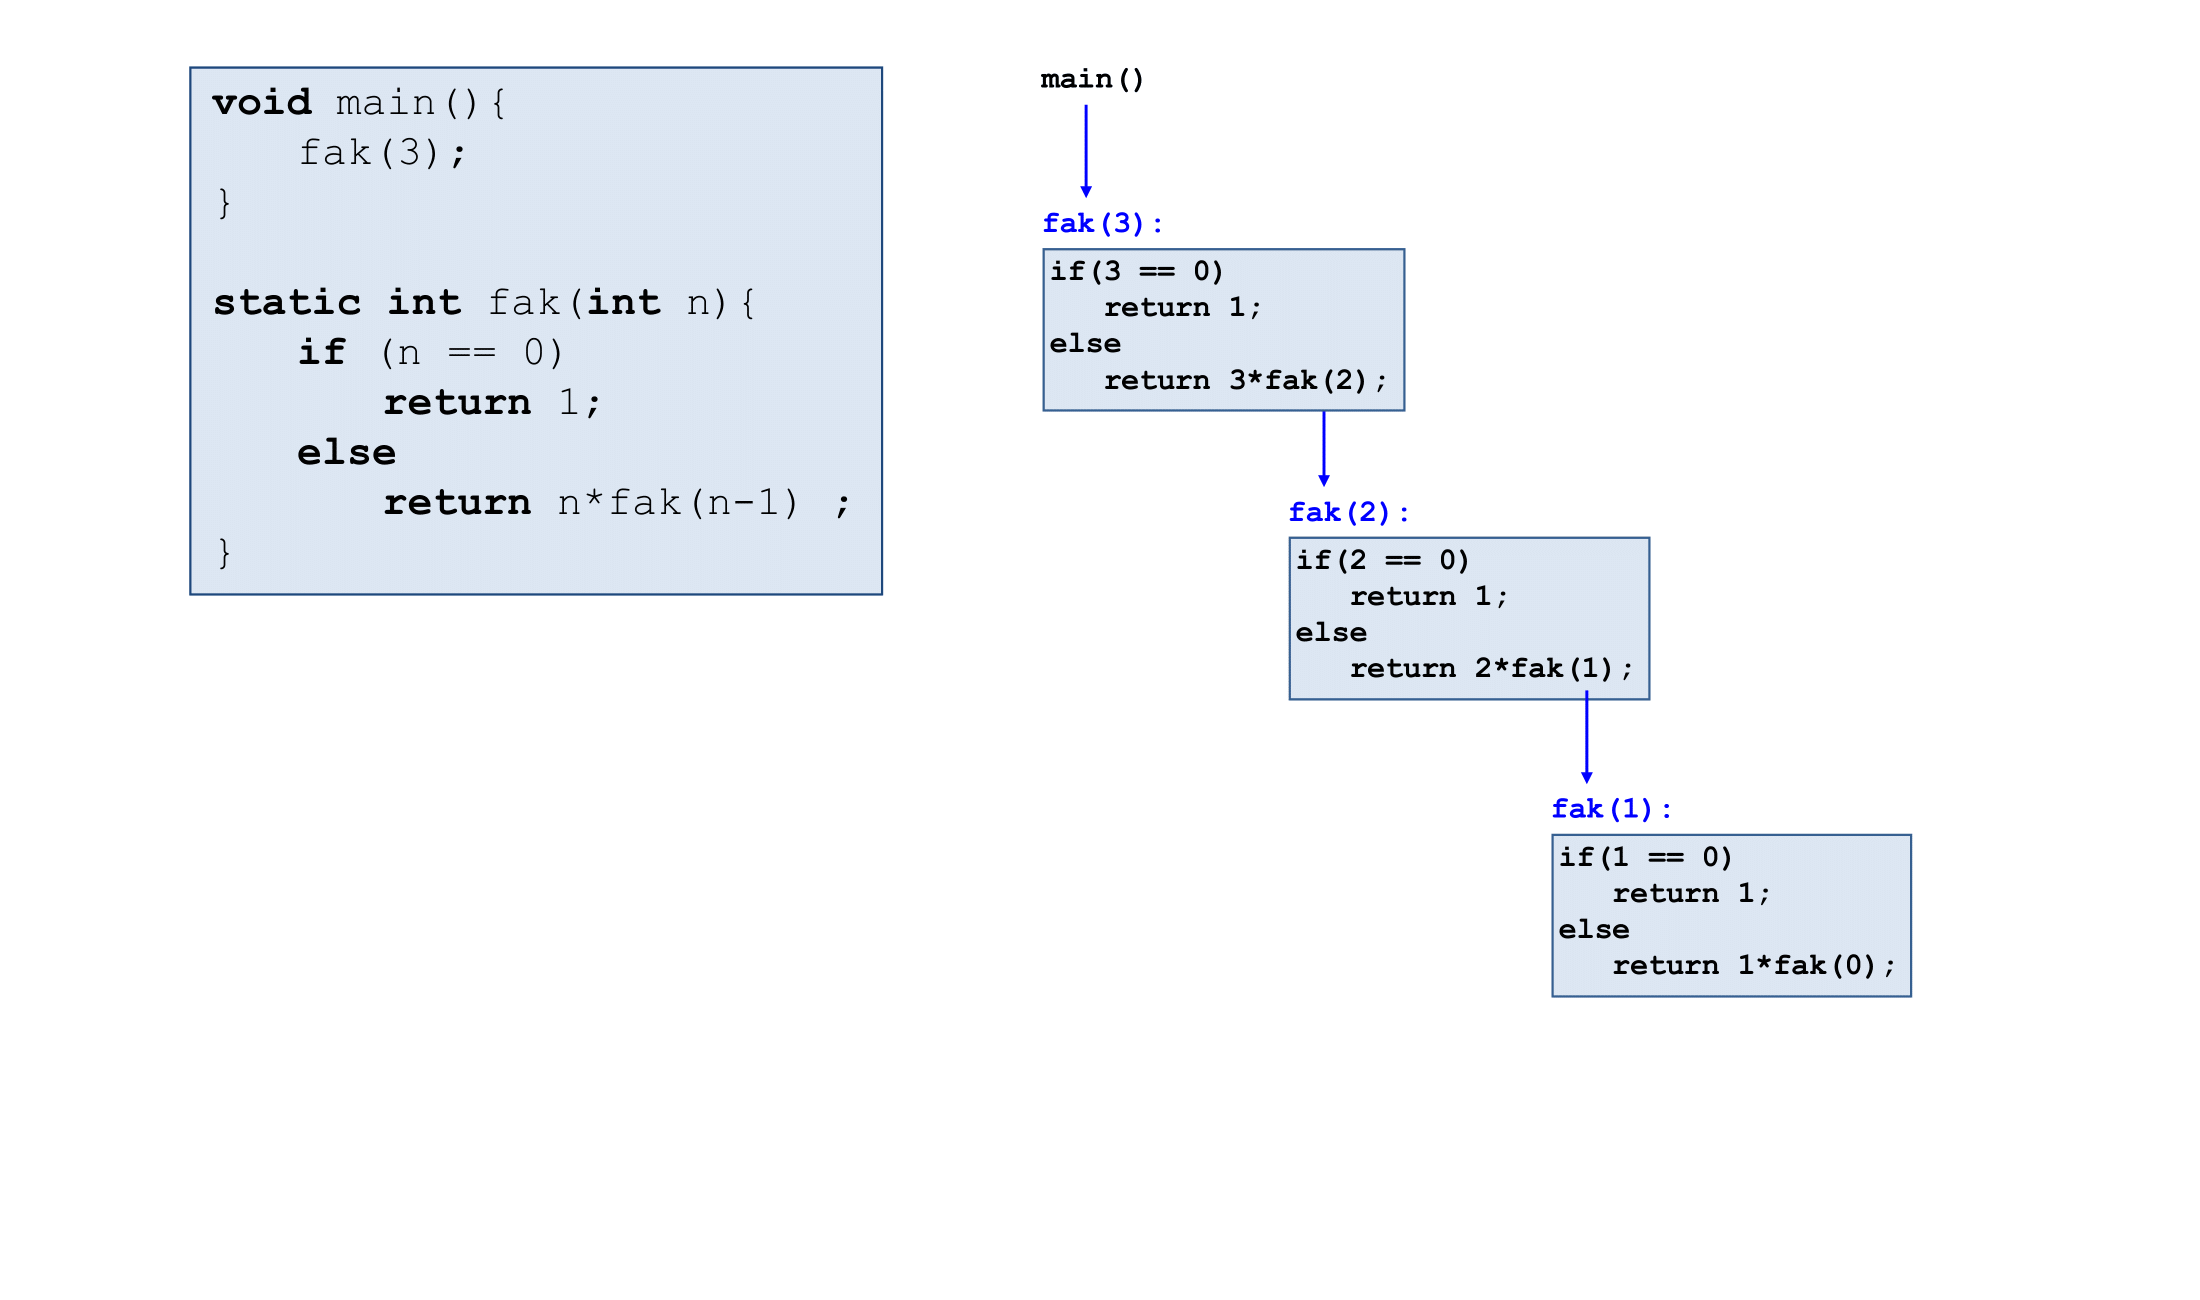
\includegraphics[width=1.1\textwidth]{rekursion anlage/07_Rekursion-06.png}
    \end{center}
\end{frame}
\begin{frame}
    \begin{center}
           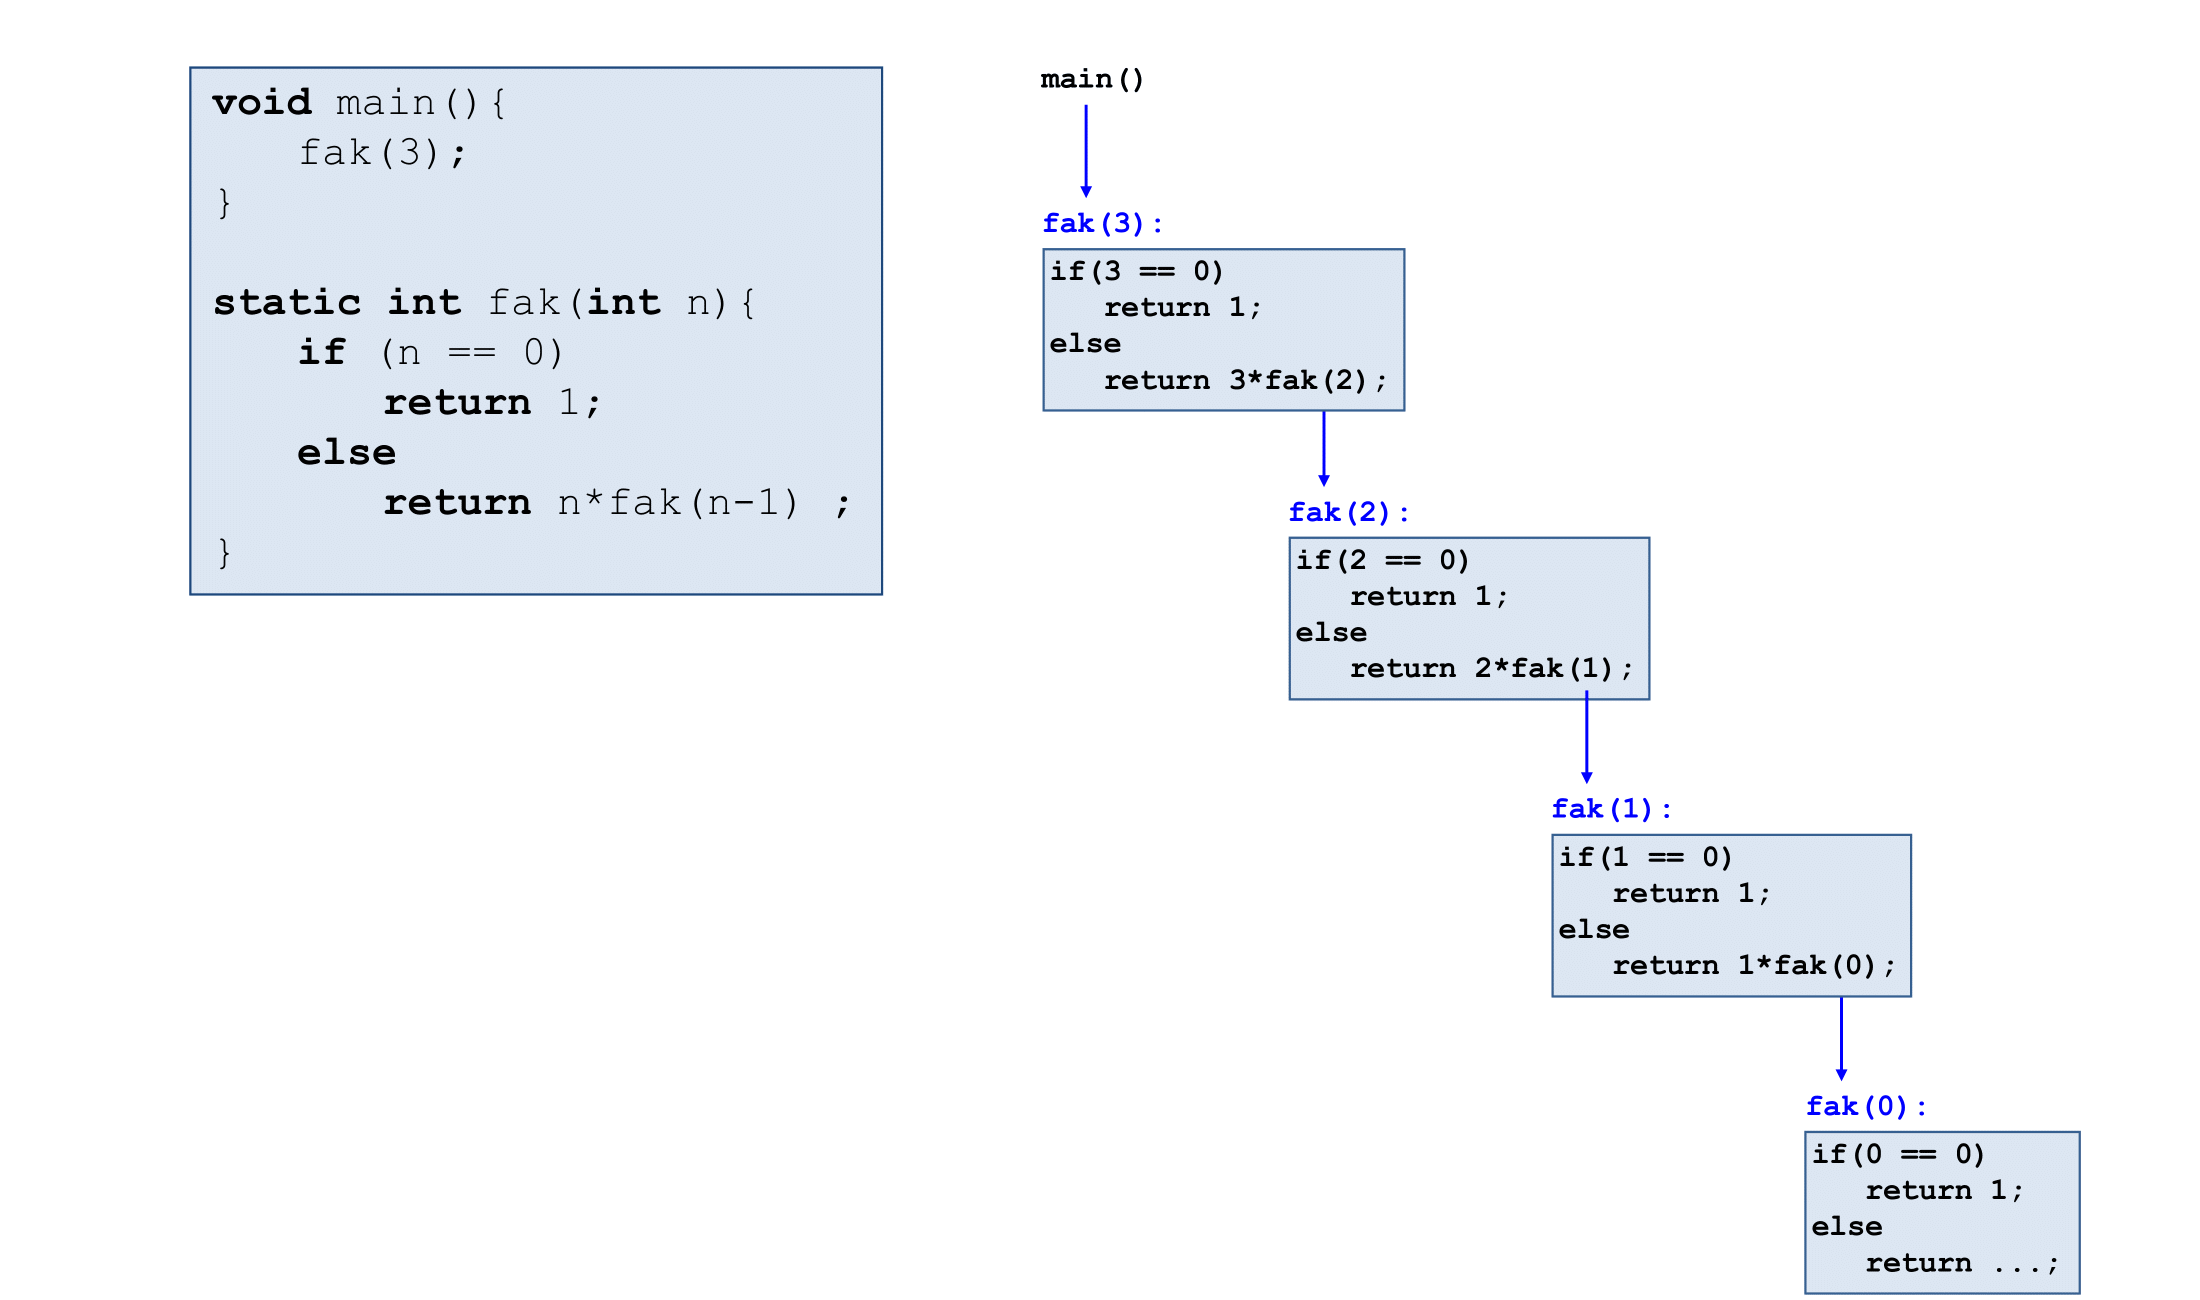
\includegraphics[width=1.1\textwidth]{rekursion anlage/07_Rekursion-07.png}
    \end{center}
\end{frame}
\begin{frame}
    \begin{center}
           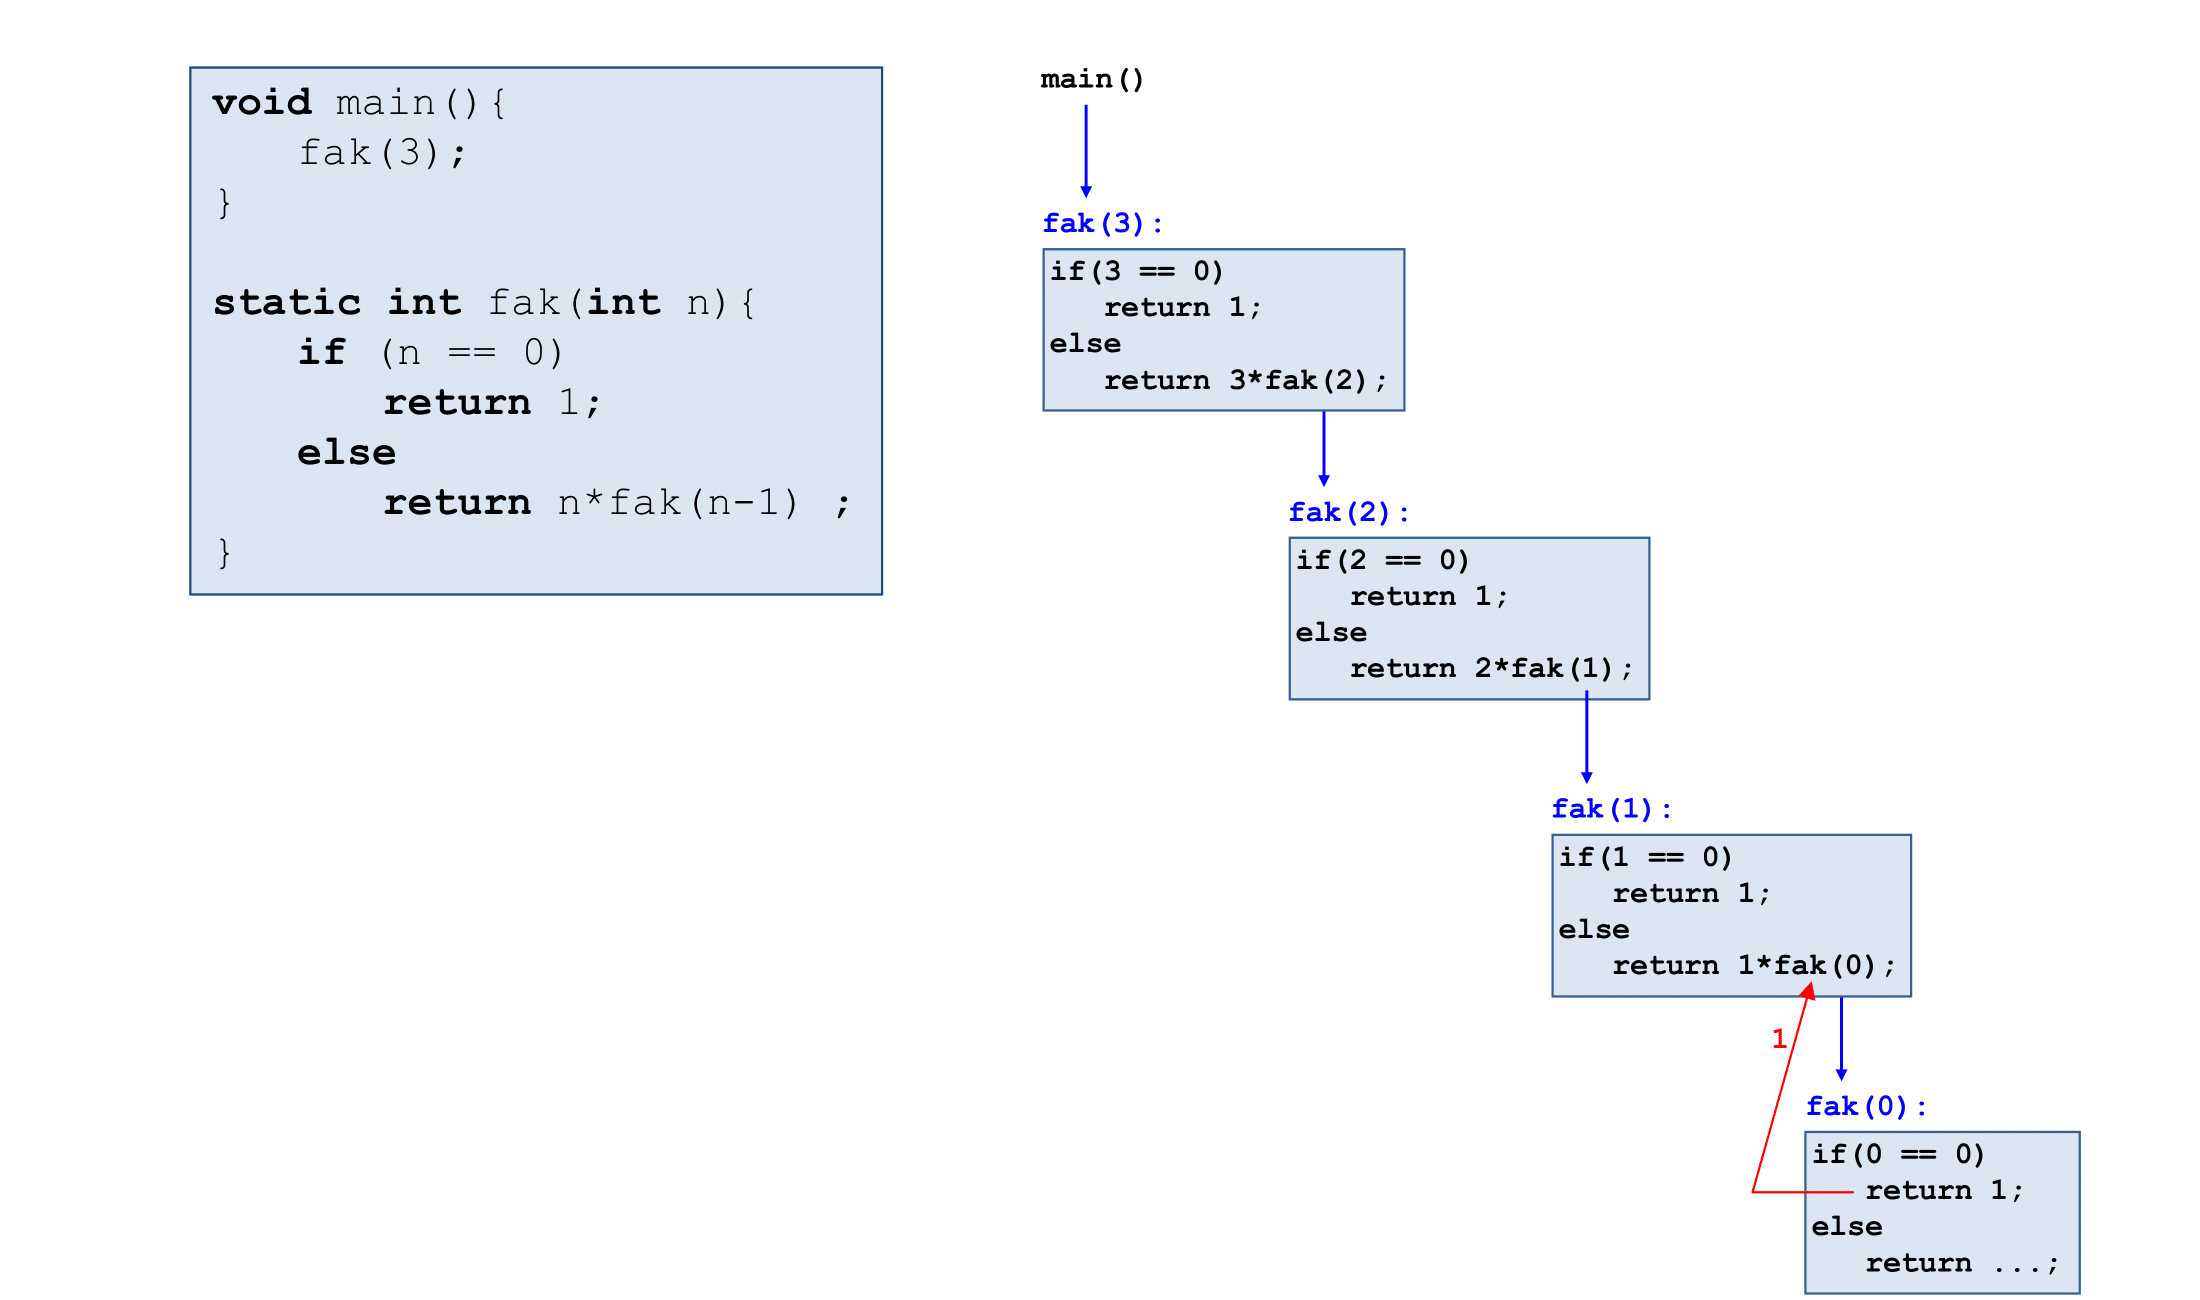
\includegraphics[width=1.1\textwidth]{rekursion anlage/07_Rekursion-08.png}
    \end{center}
\end{frame}
\begin{frame}
    \begin{center}
           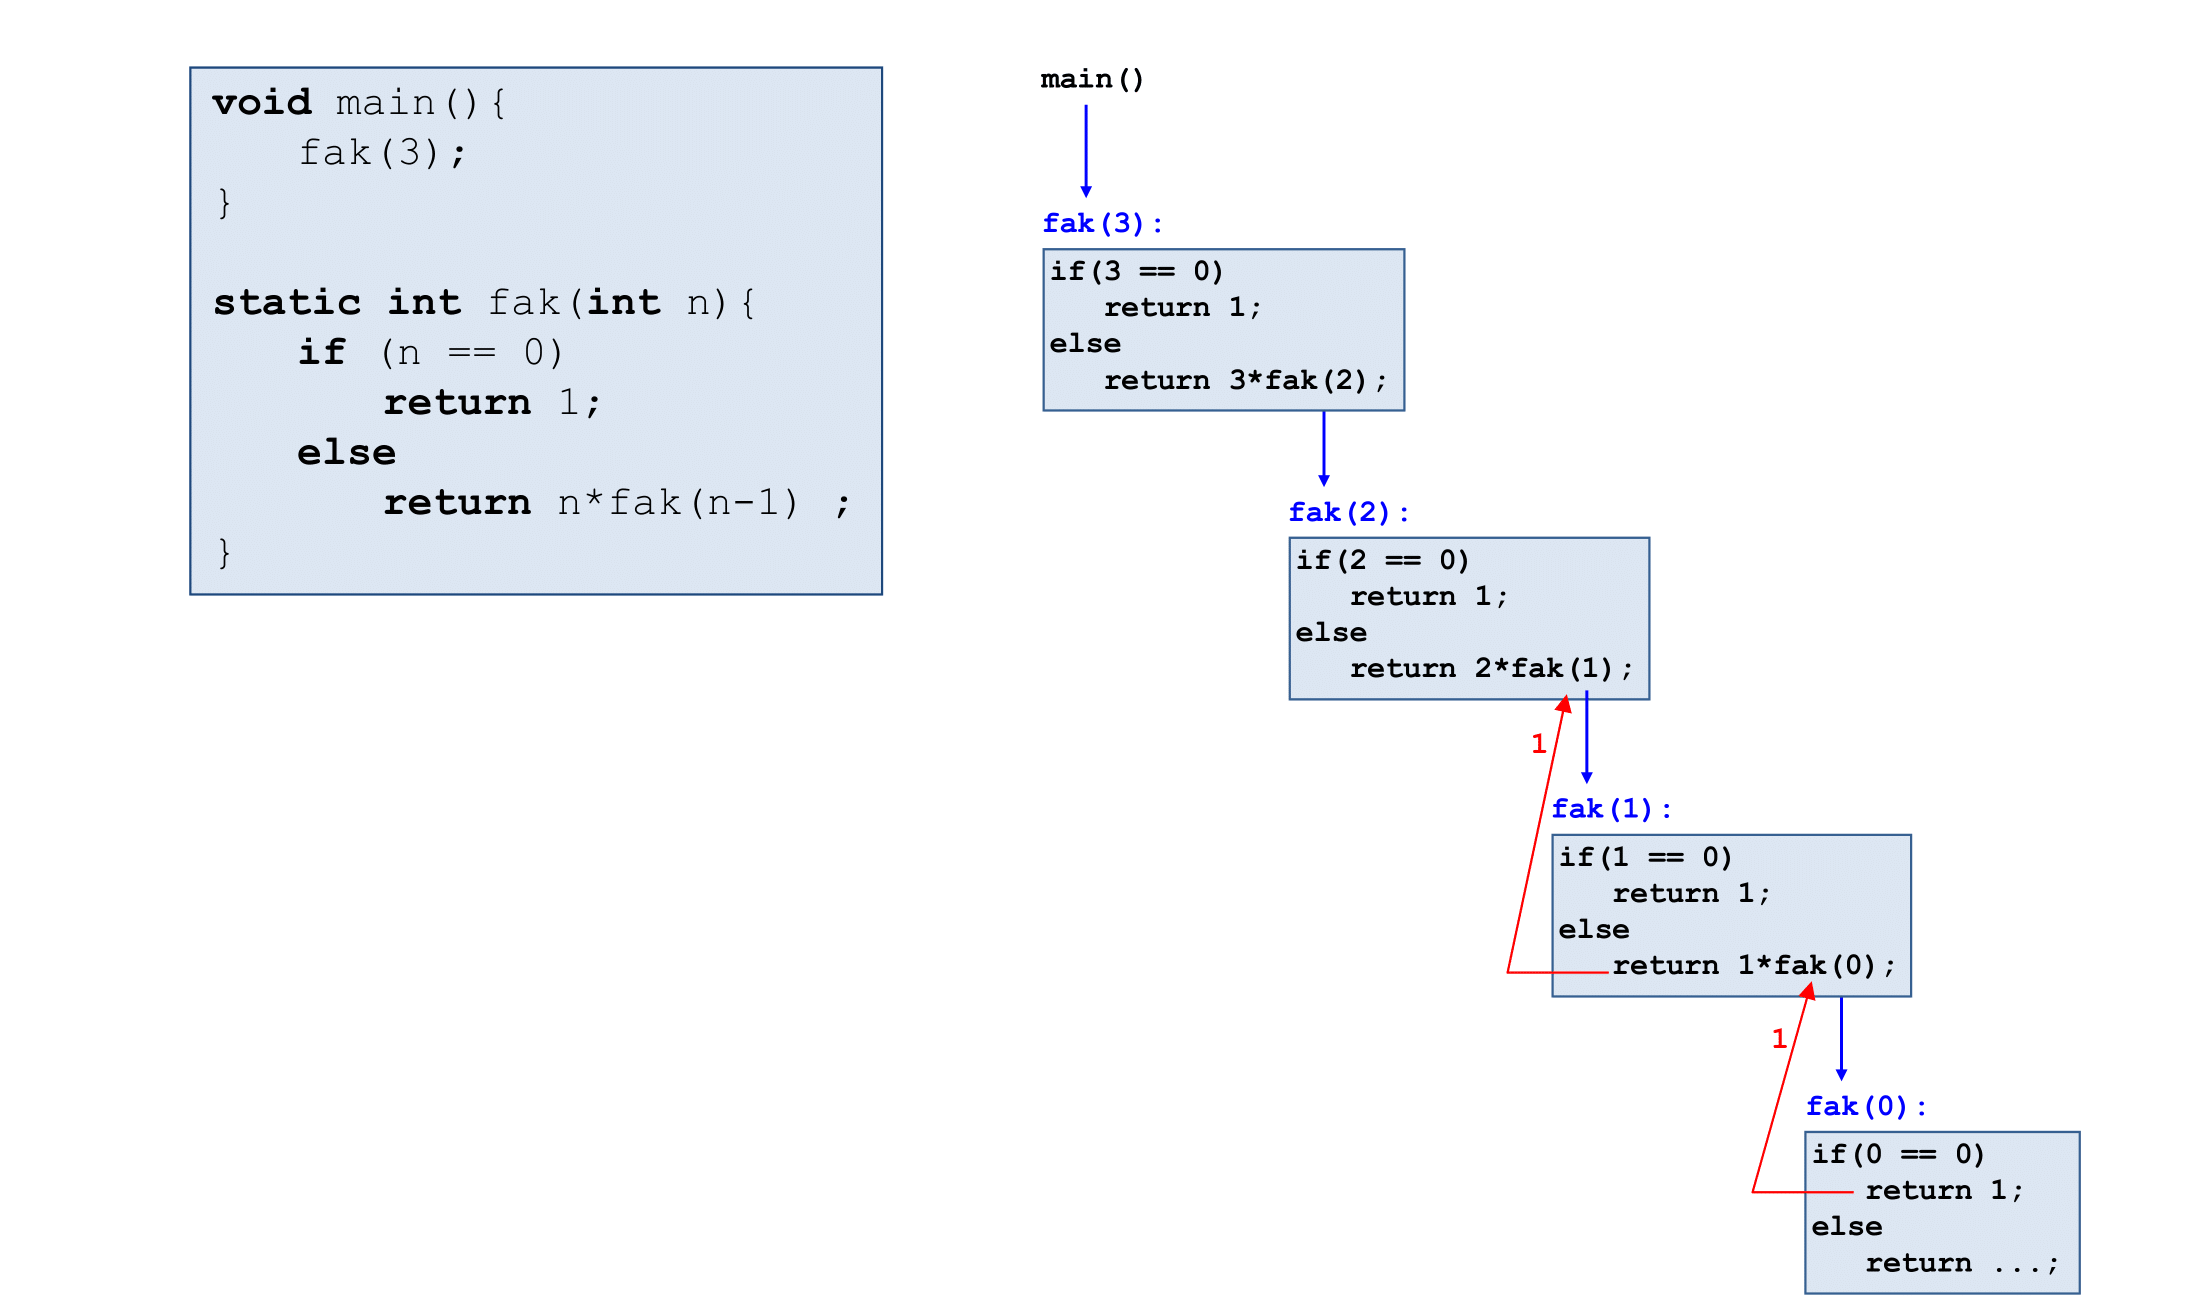
\includegraphics[width=1.1\textwidth]{rekursion anlage/07_Rekursion-09.png}
    \end{center}
\end{frame}
\begin{frame}
    \begin{center}
           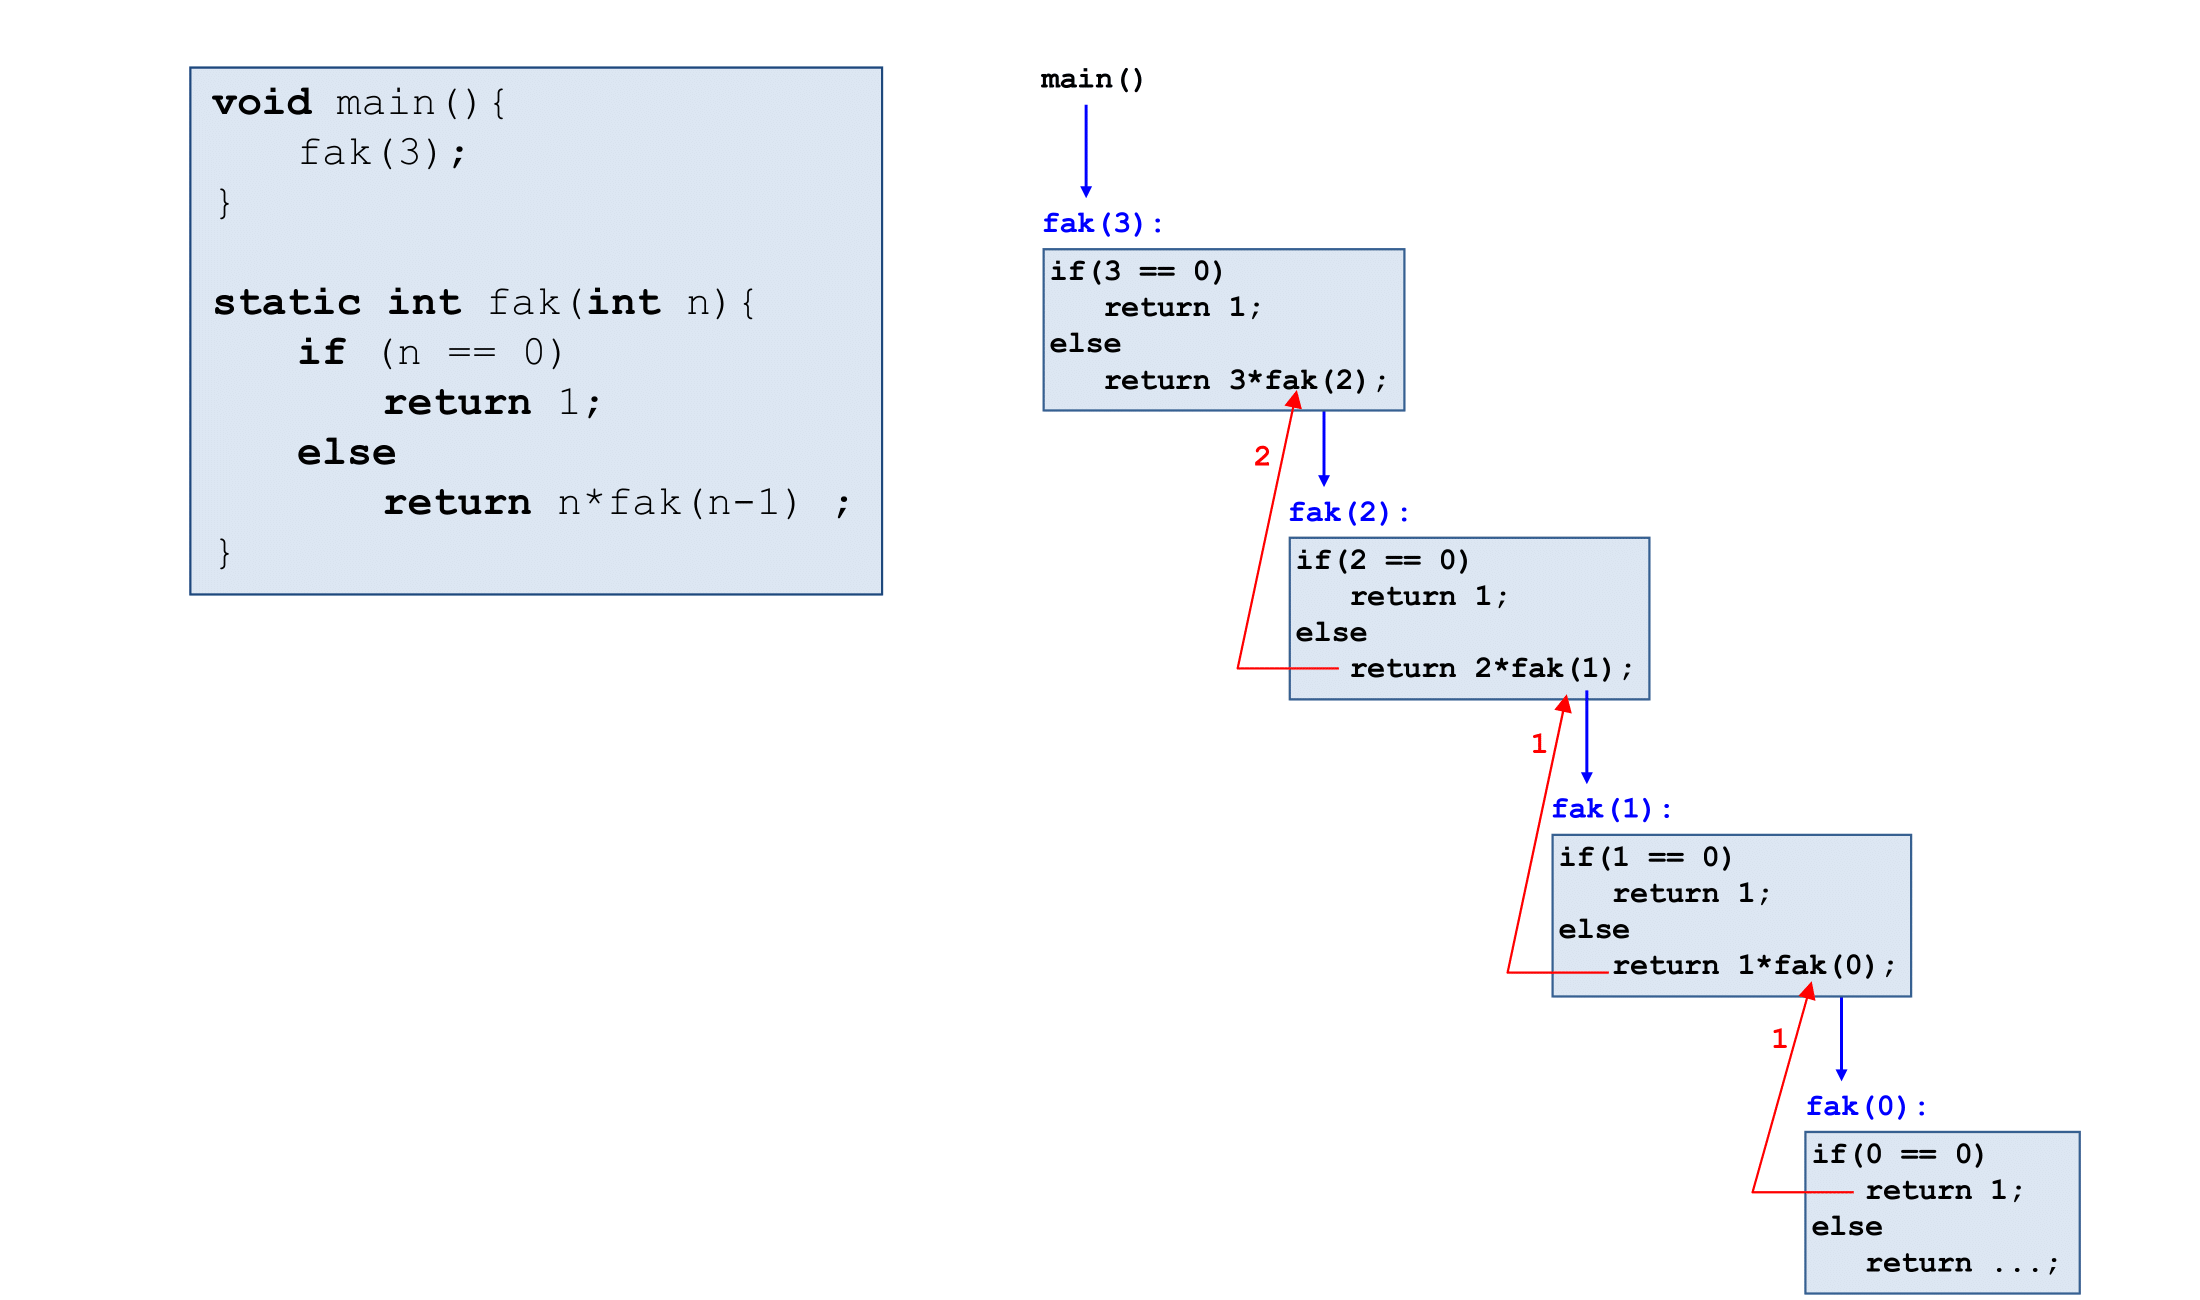
\includegraphics[width=1.1\textwidth]{rekursion anlage/07_Rekursion-10.png}
    \end{center}
\end{frame}
\begin{frame}
    \begin{center}
           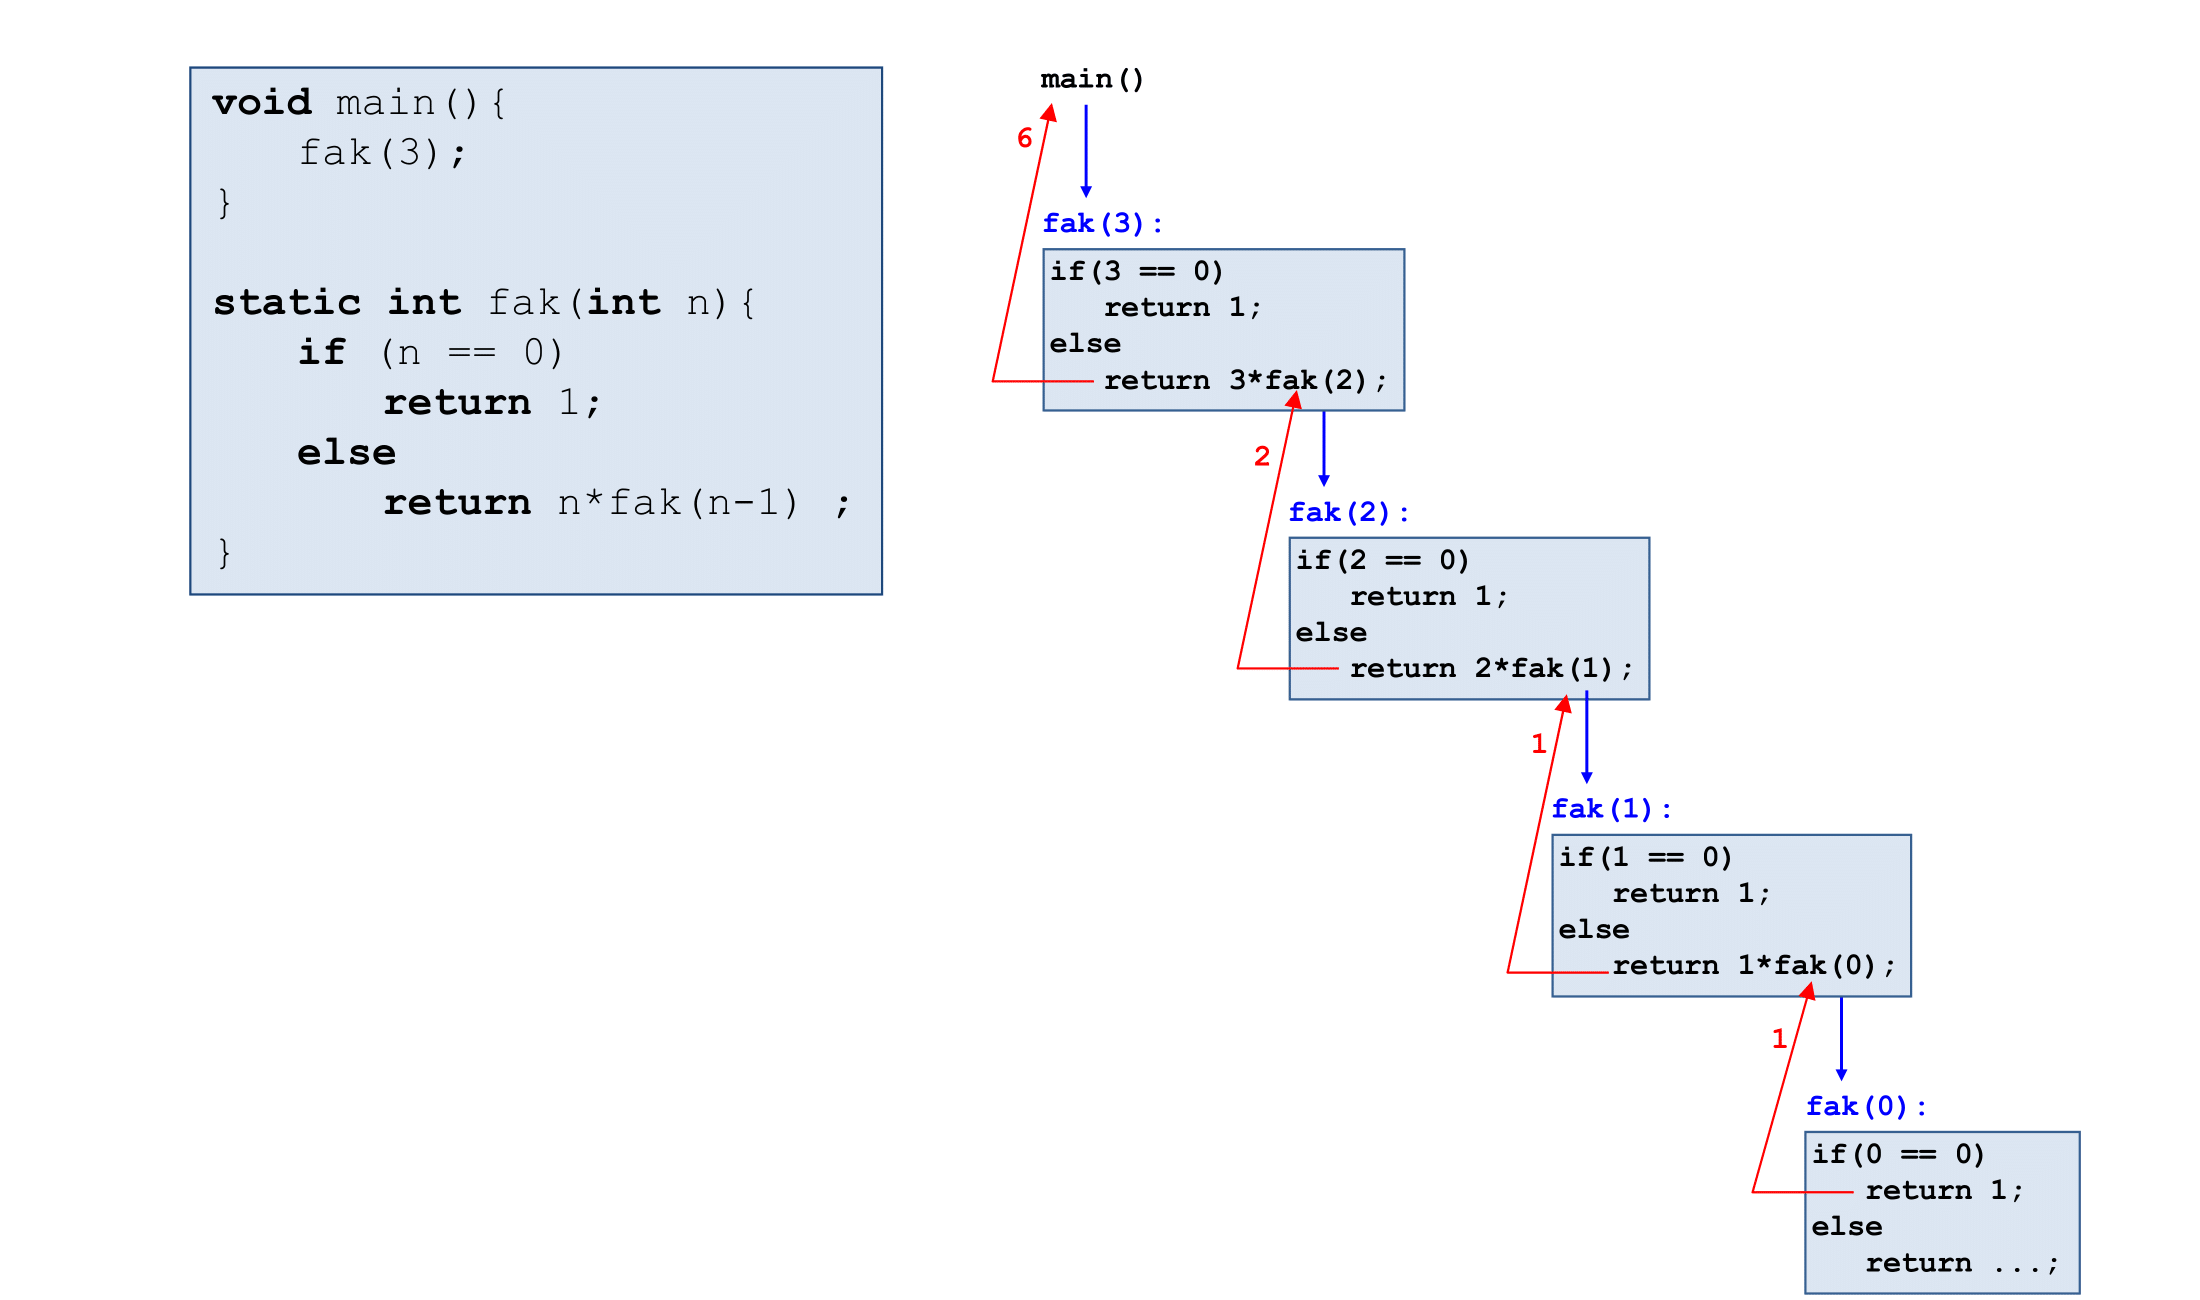
\includegraphics[width=1.1\textwidth]{rekursion anlage/07_Rekursion-11.png}
    \end{center}
\end{frame}

\section{Aufgaben}
\begin{frame}{Aufgaben}
\begin{enumerate}
  \item Die Türme von Hanoi
  \item Die Fibonacci-Folge 
  \item Zusäzliche aufgabe%Name nicht fest
\end{enumerate}
\end{frame}
\begin{frame}{Die Türme von Hanoi}
\begin{flushleft} 
    \textmd{\small
    Vermutlich wurde das Spiel 1883 vom französischen Mathematiker Édouard Lucas erfunden. 
    Er dachte sich dazu die Geschichte aus, dass indische Mönche im großen Tempel zu Benares, 
    im Mittelpunkt der Welt, einen Turm aus 64 goldenen Scheiben versetzen müssten, 
    und wenn ihnen das gelungen sei, wäre das Ende der Welt gekommen.
    }
\end{flushleft}
	
\end{frame}

\begin{frame}
\begin{figure}
    \centering
    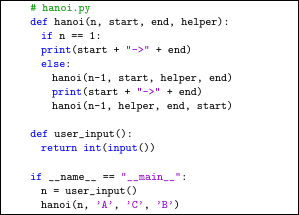
\includegraphics[width=0.8\textwidth]{code/hanoi_code.png}
\end{figure}
\end{frame}


\begin{frame}{Die Fibonacci-Folge}
    Die Fibonacci-Zahlen sind eine berühmte Folge natürlicher Zahlen, die in vielen Bereichen der Mathematik und Naturwissenschaften eine besondere Bedeutung haben. Sie wurden vom italienischen Mathematiker Leonardo von Pisa, auch bekannt als \emph{Fibonacci}, im Jahr 1202 
\end{frame}
\begin{frame}
\frametitle{Die Fibonacci-Folge}

Die Fibonacci-Folge wird \textit{rekursiv} definiert:
\[
a_n = 
\begin{cases}
1, & \text{für } n = 1 \\
1, & \text{für } n = 2 \\
a_{n-1} + a_{n-2}, & \text{für } n > 2
\end{cases}
\]
    Diese einfache rekursive Struktur führt zu einer faszinierenden Folge, die oft in der Natur und in mathematischen Zusammenhängen auftaucht, wie in der Verteilung von Blättern, in Spiralmustern, und in Wachstumsprozessen.

\end{frame}
\begin{frame}{Fibonacci-Zahl in der Natur}
    \begin{columns}
        \begin{column}{0.5\textwidth}
        \small{
            \text{Viele Samenköpfe, Tannenzapfen und }\\
            \text{Früchte zeigen spiralförmige Muster,}\\
            \text{die beim Zählen Fibonacci-Zahlen}
            \\ \text{ausdrücken. Schaut man auf die Spiralen n}
            \\ \text{der Same im Zentrum einer Sonnenblume,}
            \\ \text{erkennt man Muster, die sich nach links}\\ \text{und rechts winden.}\\ \text{Wenn man diese Spiralen zählt,}\\
            \text{ergibt die Summe eine Fibonacci-Zahl.}}
        \end{column}
        \begin{column}{0.5\textwidth}
            \centering
           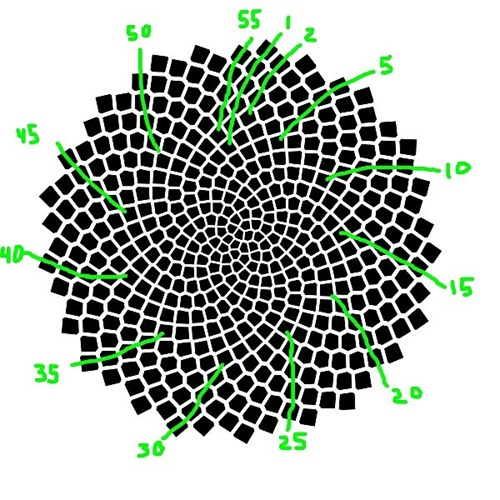
\includegraphics[width=1\textwidth]{fibonacci image.png}
        \end{column}
    \end{columns}
    \hfill \tiny Quelle: { https://momath.org/home/fibonacci-numbers-of-sunflower-seed-spirals/}
\end{frame}


\begin{frame}
    \begin{center}
           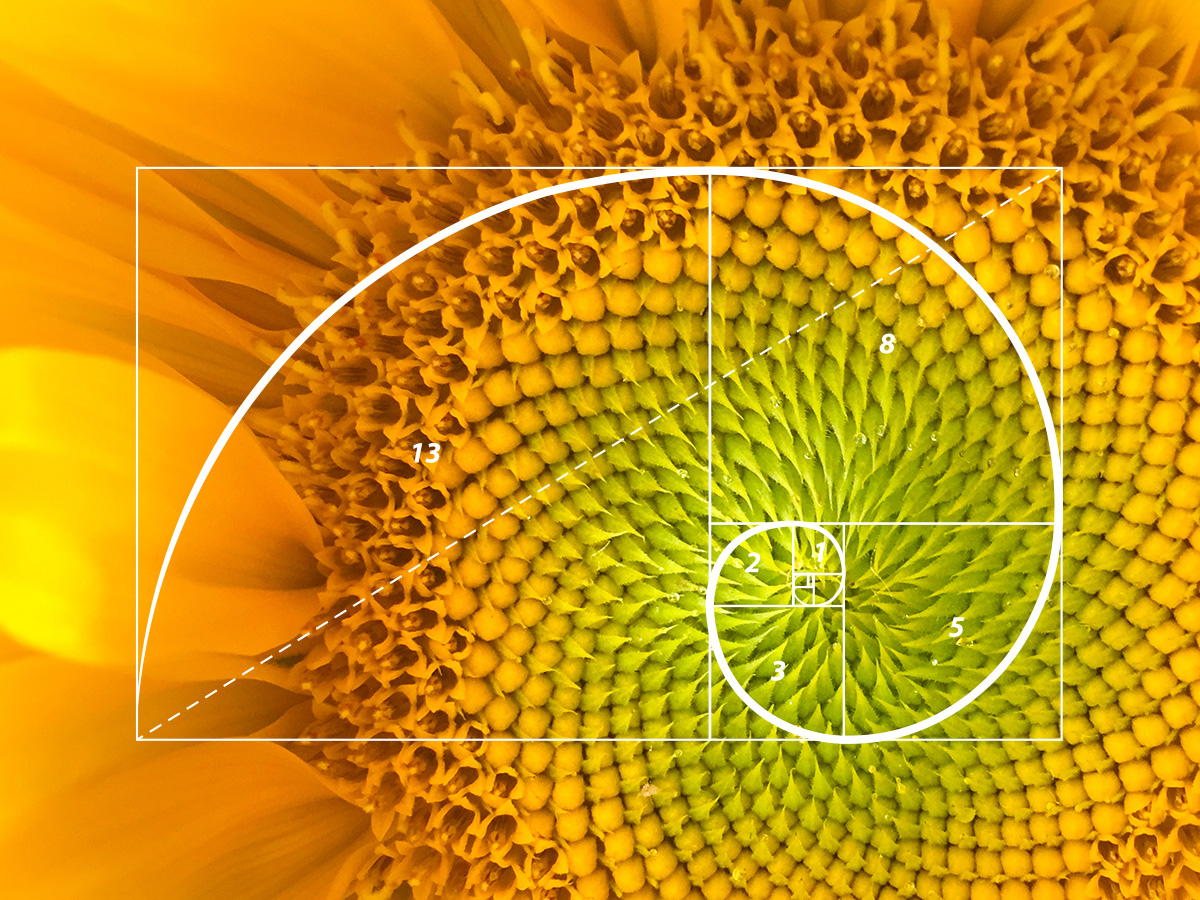
\includegraphics[width=0.5\textwidth]{sonnenblum.png}
    \end{center}
     \vspace{1em}

\end{frame}


\begin{frame}
    \begin{enumerate}
        \item \textbf{Nachteile der Rekursiven Form:}
        \begin{itemize}
            \item Um einen Term zu berechnen, müssen alle vorherigen Terme berechnet werden.
            \item Hoher Rechenaufwand bei großen \( n \), was zu ineffizientem Ressourcenverbrauch führt.
            \item Besonders in der Programmierung kann dies zu langen Berechnungszeiten führen.
        \end{itemize}
        
        \item \textbf{Vorteile der Geschlossenen Form:}
        \begin{itemize}
            \item Direkte Berechnung von \( a_n \), ohne vorherige Terme berechnen zu müssen.
            \item Spart Rechenzeit und Ressourcen, besonders bei großen \( n \).
            \item Sehr effizient für schnelle und ressourcenschonende Berechnungen.
        \end{itemize}
    \end{enumerate}
\end{frame}


\begin{frame}
\uncover<1->{
Eine geschlossene Darstellung liefert die Formel von Moivre-Binet:
\[
a_n = \frac{1}{\sqrt{5}} \left[ \left( \frac{1 + \sqrt{5}}{2} \right)^n - \left( \frac{1 - \sqrt{5}}{2} \right)^n \right]
\]
}
 \uncover<2->{Um die Berechnung zu vereinfachen, setzen wir \( \alpha = \frac{1 + \sqrt{5}}{2} \) und \( \beta = \frac{1 - \sqrt{5}}{2} \).
}

\end{frame}
\begin{frame}
\begin{enumerate}
    \uncover<1->{
    \begin{small}
    \item[a)] Beweisen durch vollständige Induktion:
    \end{small}
    }
    \[
    \begin{pmatrix} 0 & 1 \\ 1 & 1 \end{pmatrix}^n \cdot \begin{pmatrix} 0 \\ 1 \end{pmatrix} = \begin{pmatrix} a_n \\ a_{n+1} \end{pmatrix} \quad \text{für alle } n \in \mathbb{N}
    \]
    \uncover<2->{
    \begin{small}
    \item[b)] Rechnen Sie nach:
    \end{small}
    \begin{enumerate}[i]  
    \item
    \[\begin{pmatrix} 0 & 1 \\ 1 & 1 \end{pmatrix} \cdot \begin{pmatrix} 1 \\ \frac{1 + \sqrt{5}}{2} \end{pmatrix} = \frac{1 + \sqrt{5}}{2} \begin{pmatrix} 1 \\ \frac{1 + \sqrt{5}}{2} \end{pmatrix}
    \]
    }
    \uncover<3->{ 
    \item\[
    \begin{pmatrix} 0 & 1 \\ 1 & 1 \end{pmatrix} \cdot \begin{pmatrix} 1 \\ \frac{1 - \sqrt{5}}{2}  \end{pmatrix} = \frac{1 - \sqrt{5}}{2} \begin{pmatrix} 1 \\ \frac{1 - \sqrt{5}}{2} \end{pmatrix}
    \]
    }
    \end{enumerate}
\end{enumerate}
\end{frame}

\begin{frame}
    \begin{flushleft} 
     \uncover<1->{$\begin{pmatrix} 0 & 1 \\ 1 & 1 \end{pmatrix}  \begin{pmatrix} 1 \\ \frac{1 - \sqrt{5}}{2}  \end{pmatrix}$
    }
    \uncover<2->{$=\begin{pmatrix} \beta \\ 1+ \beta \end{pmatrix}$}
    \uncover<3->{=\beta  \begin{pmatrix} 1 \\ \frac{1}{\beta} + 1 \end{pmatrix}
    } 
    \uncover<4->{$= \beta \begin{pmatrix} 1 \\ \frac{2}{1 - \sqrt{5}}+1  \end{pmatrix}$}
    \uncover<5->{$=\beta  \begin{pmatrix} 1 \\ \frac{1 - 2\sqrt{5}+5}{2(1 - \sqrt{5})}  \end{pmatrix}$}
    \uncover<6->{$=\beta  \begin{pmatrix} 1 \\ \frac{(1 -\sqrt{5})^2}{2(1 - \sqrt{5})}  \end{pmatrix}$}
    \uncover<7->{$=\frac{1 - \sqrt{5}}{2}  \begin{pmatrix} 1 \\ \frac{1 -\sqrt{5}}{2}  \end{pmatrix}$}
    
    \end{flushleft}
    \uncover<7->{
    \hspace*{\fill} $\square$
    }
\end{frame}

\begin{frame}
\begin{enumerate}
    \begin{small}
    \item a) Beweisen Sie durch vollständige Induktion:
    \end{small}
    \[
    \begin{pmatrix} 0 & 1 \\ 1 & 1 \end{pmatrix}^n \cdot \begin{pmatrix} 0 \\ 1 \end{pmatrix} = \begin{pmatrix} a_n \\ a_{n+1} \end{pmatrix} \quad \text{für alle } n \in \mathbb{N}
    \]
    \begin{small}
    \item[b)] Rechnen Sie nach:
    \end{small}
    \begin{enumerate}[i]  
    \item
    \[\begin{pmatrix} 0 & 1 \\ 1 & 1 \end{pmatrix} \cdot \begin{pmatrix} 1 \\ \frac{1 + \sqrt{5}}{2} \end{pmatrix} = \frac{1 + \sqrt{5}}{2} \begin{pmatrix} 1 \\ \frac{1 + \sqrt{5}}{2} \end{pmatrix}
    \]
    
    \item\[
    \begin{pmatrix} 0 & 1 \\ 1 & 1 \end{pmatrix} \cdot \begin{pmatrix} 1 \\ \frac{1 - \sqrt{5}}{2}  \end{pmatrix} = \frac{1 - \sqrt{5}}{2} \begin{pmatrix} 1 \\ \frac{1 - \sqrt{5}}{2} \end{pmatrix}
    \]
    \item
    \[
     \begin{pmatrix} 0 \\ 1 \end{pmatrix} = \frac{1}{\sqrt{5}} \cdot \left[ \begin{pmatrix} 1 \\ \frac{1 + \sqrt{5}}{2} \end{pmatrix} - \begin{pmatrix} 1 \\ \frac{1 - \sqrt{5}}{2} \end{pmatrix} \right]
    \]
    
\end{enumerate}
\end{enumerate}
\end{frame}

\begin{frame}
Wir zeigen dass:
\[
\begin{pmatrix} a_n \\ a_{n+1} \end{pmatrix} = \frac{1}{\sqrt{5}} \cdot \begin{pmatrix} (\frac{1 + \sqrt{5}}{2})^n-(\frac{1 - \sqrt{5}}{2})^n \\ (\frac{1 + \sqrt{5}}{2})^{n+1}-(\frac{1 - \sqrt{5}}{2})^{n+1} \end{pmatrix} 
\]
\end{frame}

\begin{frame}
zunächst sei die Funktion $ f(x) = \frac{1}{\sqrt{5}} \cdot \left( \frac{1 + \sqrt{5}}{2} \right)^{x} $
\end{frame}
\begin{frame}
% Aufgabe3.4)a graph
\begin{tikzpicture}
\uncover<1->{
% Main plot
\begin{axis}[
    width=10cm, height=7cm,
    xmin=0, xmax=8,
    ymin=0, ymax=15,
    legend style={font=\small},
    legend pos=north west,
    ymajorgrids=true,
    grid style=dashed,
    title={\small Graph von :$ f(x) = \frac{1}{\sqrt{5}} \cdot \left( \frac{1 + \sqrt{5}}{2} \right)^{x} $}
]

% Plot f(x)
\addplot[
    domain=-1:20, 
    samples=100, 
    color=blue,
    thick
]
{(1/sqrt(5)) * ((1 + sqrt(5))/2)^x};
\addlegendentry{f(x)}
]
\end{axis}
}
\uncover<2->{
% Main plot
\begin{axis}[
    width=10cm, height=7cm,
    xmin=0, xmax=8,
    ymin=0, ymax=15,
    legend style={font=\small},
    legend pos=north west,
    ymajorgrids=true,
    grid style=dashed,
]
% Plot f(x)
\addplot[
    domain=-1:20, 
    samples=100, 
    color=blue,
    thick
]
{(1/sqrt(5)) * ((1 + sqrt(5))/2)^x};
\addlegendentry{f(x)}

% Plot a_n
\addplot[
    only marks,
    mark=*,
    mark size=1.5pt,
    color=red
]
coordinates {
    (1,1) (2,1) (3,2) (4,3) (5,5) (6,8) (7,13)  
};
\addlegendentry{$a_n$}
\end{axis}
}
\end{tikzpicture}
 \vspace{1em}
 \href{https://www.desmos.com/calculator/cc8ypq4bb9?lang=de}{Desmos}
\end{frame}

\begin{frame}
\begin{flushleft}
\textbf{Aufgabe 3.4.i):} \\[1em]
Zu zeigen ist, dass der Abstand zwischen \( f(n) \) und \( a_n \) immer kleiner wird, wobei \( n \in \mathbb{N} \) ist.\\ bzw.
\\
\[
\lim_{n \to \infty} |f(n) - a_n|=0
\]
\end{flushleft}
\end{frame}
\begin{frame}
\textbf{Aufgabe 3.4.ii):} \\[1em]
\[
a_n = \left\lfloor f(n) + 0.5 \right\rfloor \quad \text{für alle } n \in \mathbb{N}
\]
Dabei ist \( \left\lfloor \cdot \right\rfloor \) die Abrundungsfunktion. \( \left\lfloor \cdot \right\rfloor \) wird auch als Gauß-Klammer bezeichnet und die Formel \( \left\lfloor \cdot + 0.5 \right\rfloor \) beschreibt das übliche Runden auf die nächste ganze Zahl.

\end{frame}



\begin{frame}
\textbf{Aufgabe 3.5):} \\[1em]

\begin{center}
       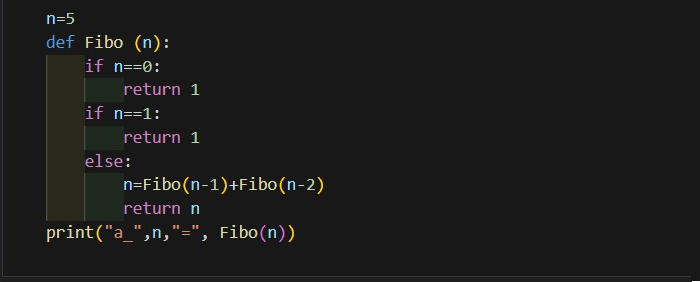
\includegraphics[width=1\textwidth]{code/3.5/3.5-00.png}
\end{center}
\end{frame}

\begin{frame}
\begin{center}
       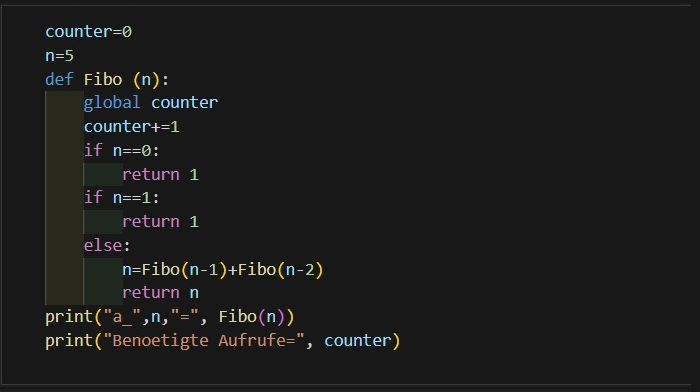
\includegraphics[width=1\textwidth]{code/3.5/3.5-01.png}
\end{center}
\end{frame}
\begin{frame}
\begin{center}
       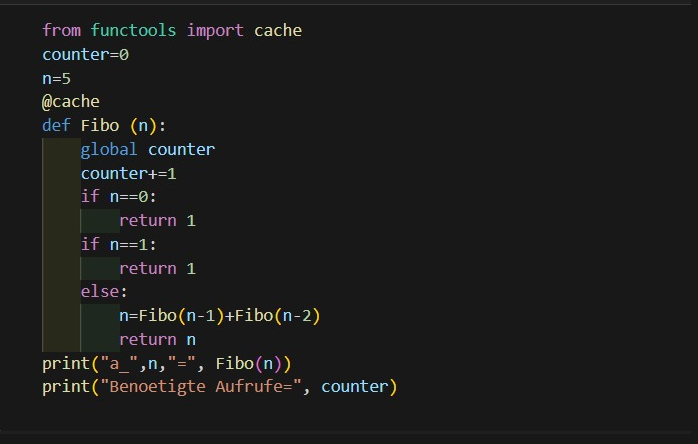
\includegraphics[width=1\textwidth]{code/3.5/3.5-02.png}
\end{center}
\end{frame}
\begin{frame}
\noindent \textbf{Aufgabe 3.6} \\
Die Zahl 
\[
\frac{1 + \sqrt{5}}{2} \approx 1.61803
\]
wird als Goldener Schnitt bezeichnet.

Zeigen Sie mit Hilfe der Formel von Moivre-Binet, dass
\[
\lim_{n \to \infty} \frac{a_{n+1}}{a_n} = \frac{1 + \sqrt{5}}{2}.
\]


\end{frame}

\begin{frame}{Goldene Schnitt}

\begin{tikzpicture}
    \uncover<1->{ 
        \draw[fill=blue!20] (0,0.75) rectangle (0.25,1);
        \node at (.25/2, 1.75/2) {\scriptsize 1}; 
    }

    \uncover<2->{ 
        \draw[fill=green!20] (0,0.5) rectangle (0.25,0.75);
        \node at (0.25/2,1.25/2) {\scriptsize 1}; 
    }

    \uncover<3->{ 
        \draw[fill=red!20] (0.25,0.5) rectangle (0.75,1);
        \node at (0.5,0.75) {\scriptsize 2};
    }
    
    \uncover<4->{ 
        \draw[fill=orange!20] (0,1) rectangle (0.75,1.75);
        \node at (0.75/2, 2.75/2) {\small 3}; 
    }
    
    \uncover<5->{ 
        \draw[fill=purple!20] (-1.25,0.5) rectangle (0,1.75);
        \node at (-1.25/2, 1.15) {\small 5}; 
    }
    
    \uncover<6->{ 
        \draw[fill=cyan!20] (-1.25,-1.5) rectangle (1.5/2,1/2);
        \node at (-0.25, -0.5) {8}; 
    }
    \uncover<7->{ 
        \draw[fill=yellow!20] (0.75,-1.5) rectangle (4,1.75);
        \node at (4.75/2, 0.25/2) {13}; 
    }
    \uncover<11->{
     \draw [red] (0.75,-1.5)  arc[start angle=270, end angle=360, radius=3.25cm];
     \draw [red] (-1.25,0.5)  arc[start angle=180, end angle=270, radius=2cm];
     \draw [red] (0,1.75)  arc[start angle=90, end angle=180, radius=1.25cm];
     \draw [red] (0.75,1)  arc[start angle=0, end angle=90, radius=0.75cm];
     \draw [red] (0.25,0.5)  arc[start angle=270, end angle=360, radius=0.5cm];
     \draw [red] (0,0.75)  arc[start angle=180, end angle=270, radius=0.25cm];
     \draw [red] (0.25,1)  arc[start angle=90, end angle=180, radius=0.25cm];
    }
\end{tikzpicture}
\\

\uncover<8->{
Die fläche des Rechteckes
\\
 
$1^2+1^2+2^2+3^2+5^2+8^2+13^2$\\
}
\uncover<9->{
Aber auch :
\\
$13\times(8+13)$
}
\uncover<10->{
$=13 \times 21$
}

\end{frame}
\begin{frame}
    \textbf{Der Goldene Schnitt}

   \begin{center}
        \only<1>{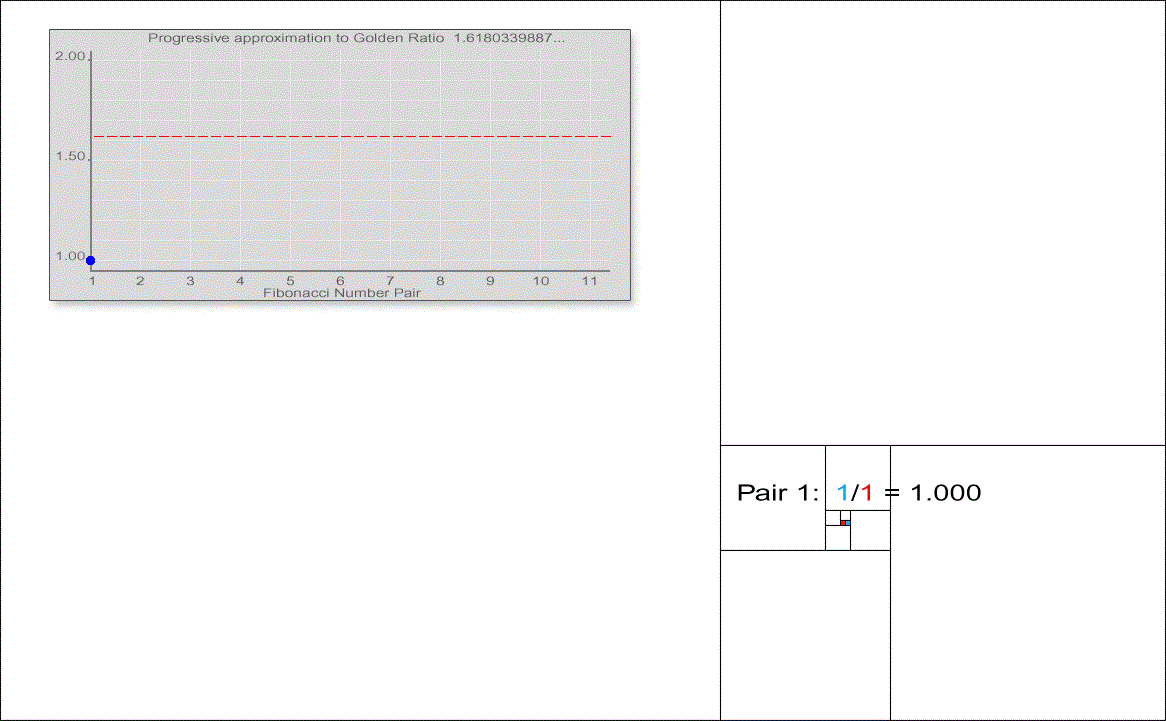
\includegraphics[width=0.9\textwidth]{goldenschnitt/frame_00.png}}
        \only<2>{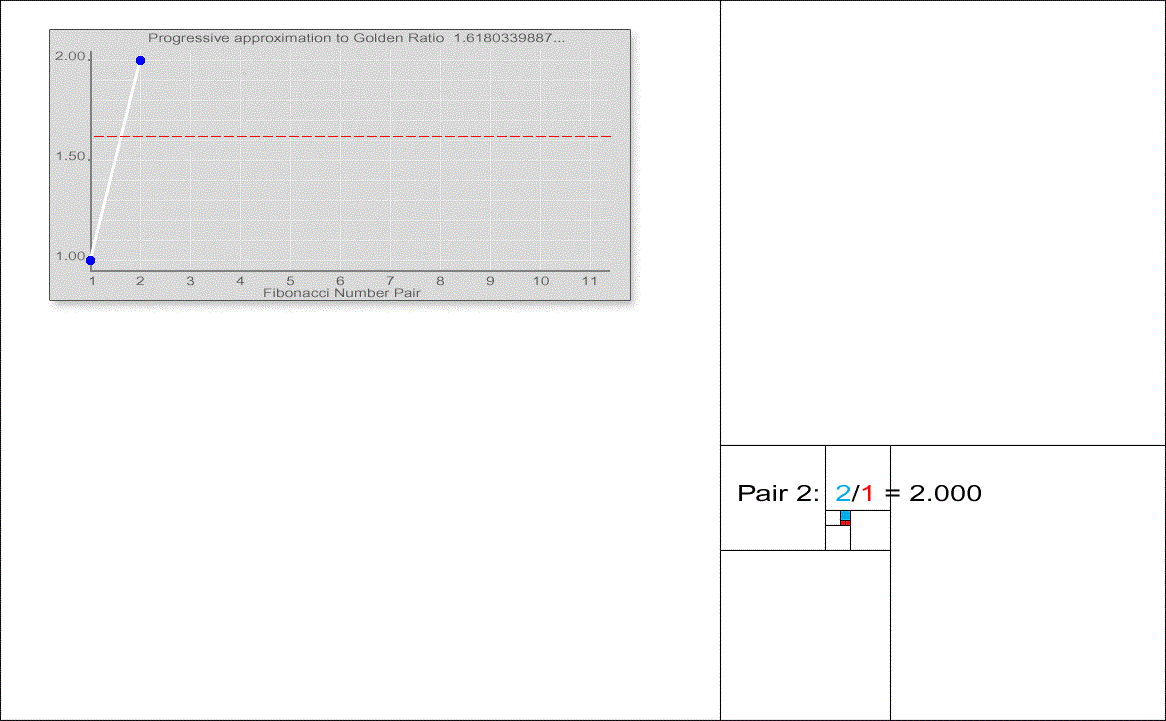
\includegraphics[width=0.9\textwidth]{goldenschnitt/frame_01.png}}
        \only<3>{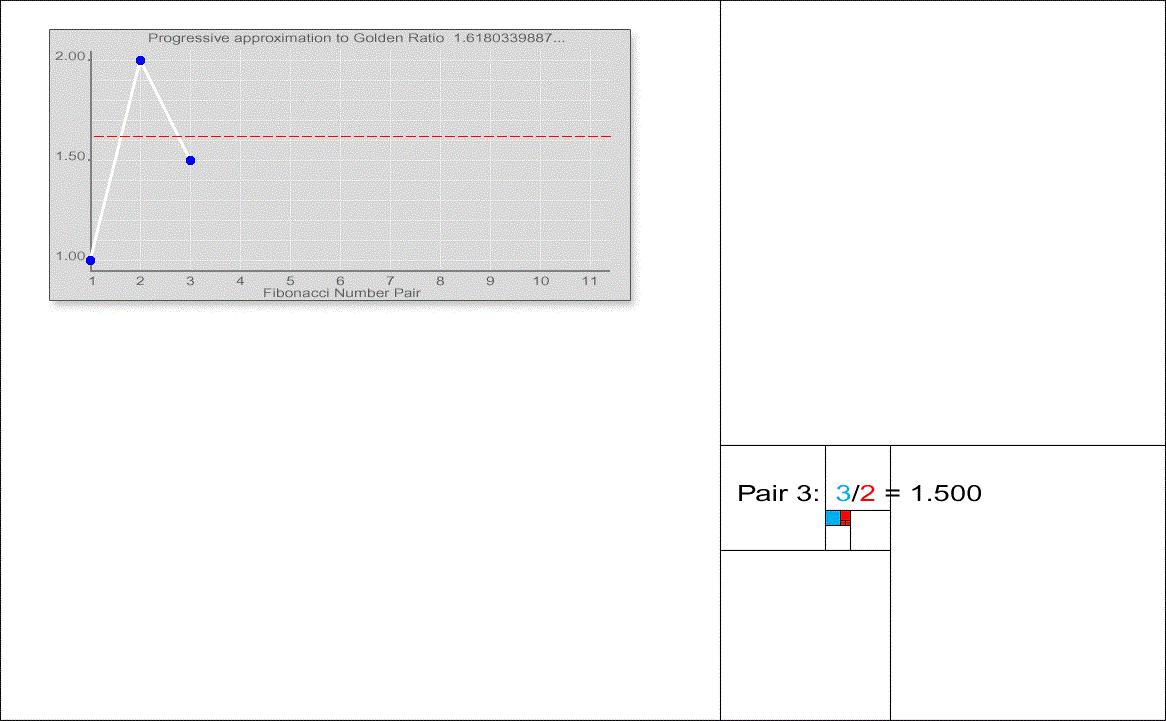
\includegraphics[width=0.9\textwidth]{goldenschnitt/frame_02.png}}
        \only<4>{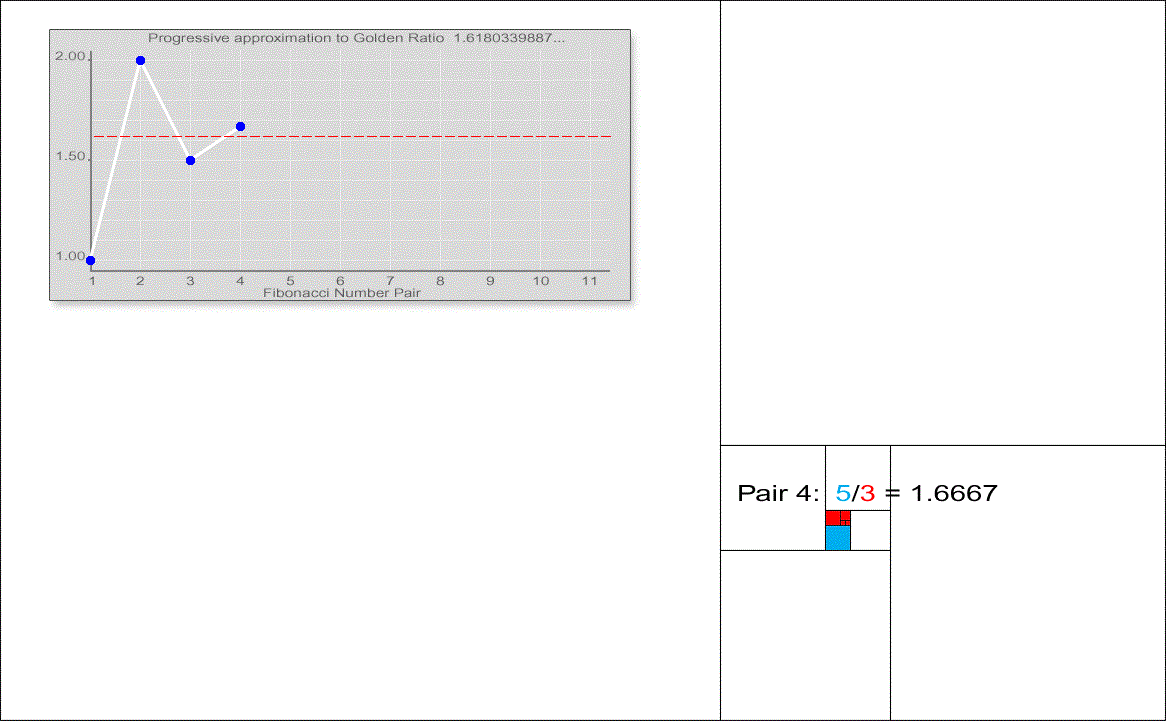
\includegraphics[width=0.9\textwidth]{goldenschnitt/frame_03.png}}
        \only<5>{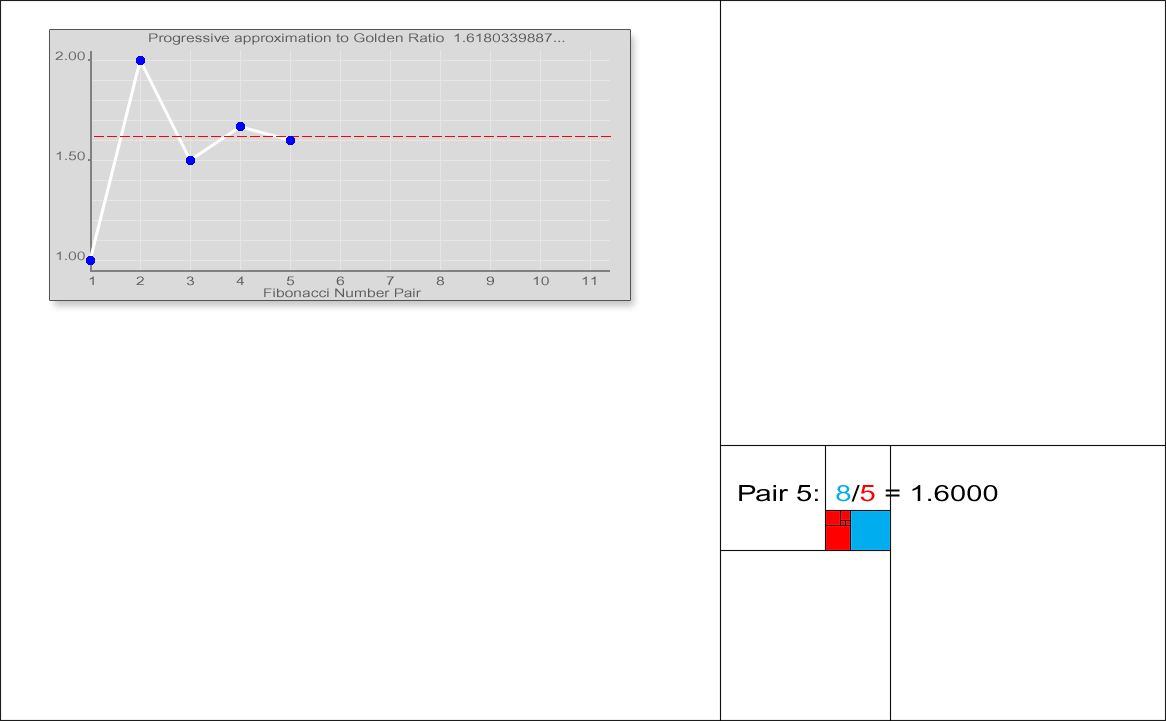
\includegraphics[width=0.9\textwidth]{goldenschnitt/frame_04.png}}
        \only<6>{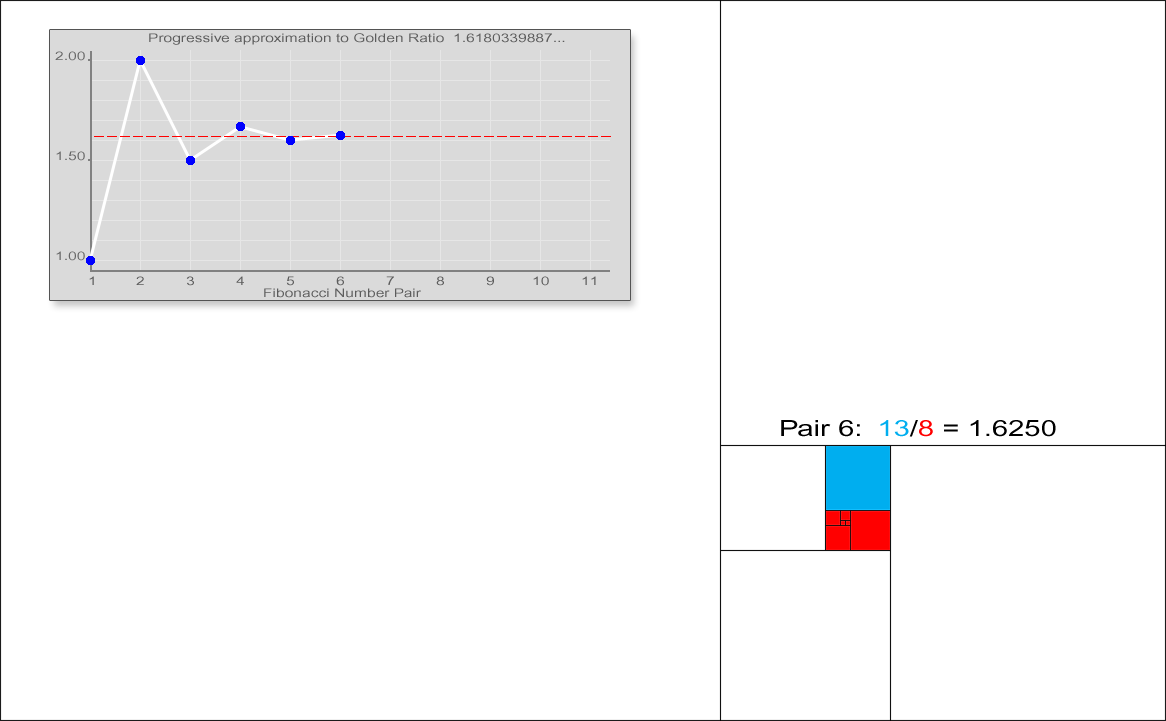
\includegraphics[width=0.9\textwidth]{goldenschnitt/frame_05.png}}
        \only<7>{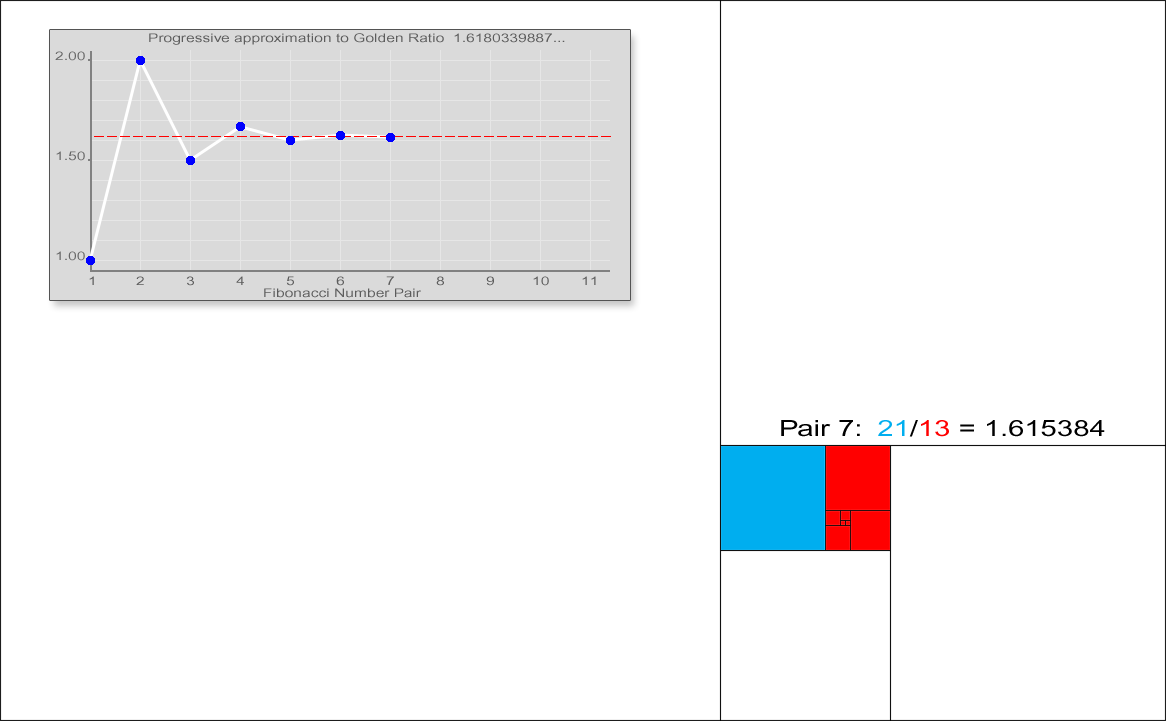
\includegraphics[width=0.9\textwidth]{goldenschnitt/frame_06.png}}
        \only<8>{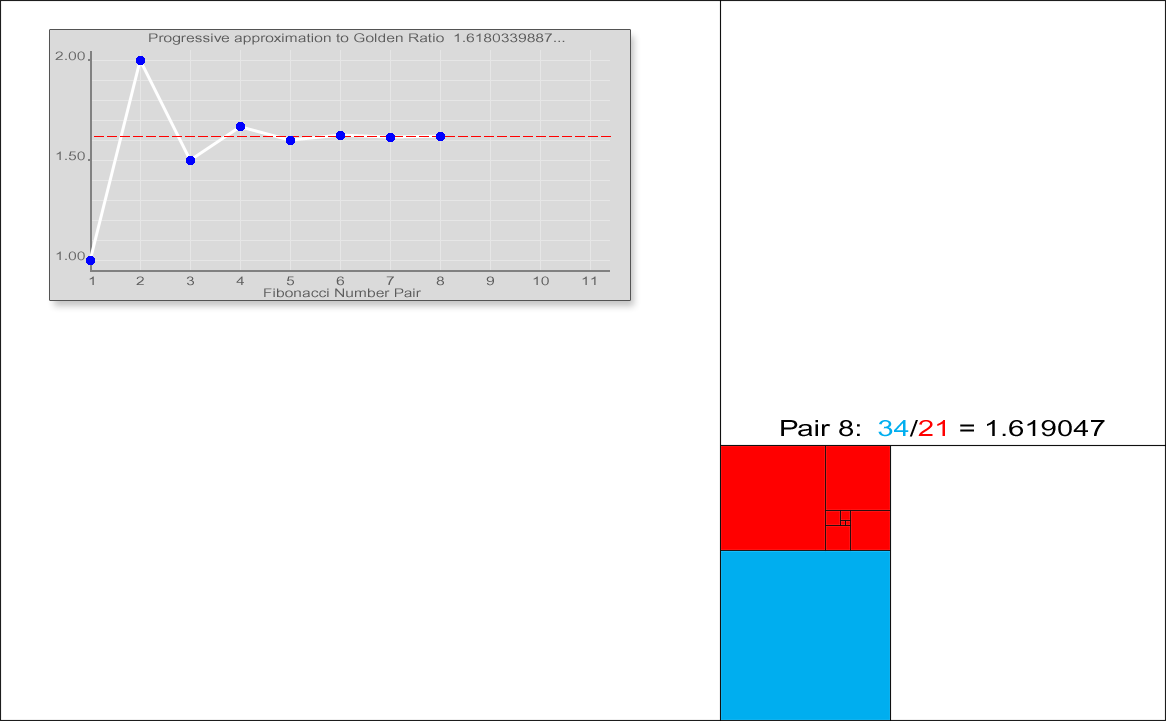
\includegraphics[width=0.9\textwidth]{goldenschnitt/frame_07.png}}
        \only<9>{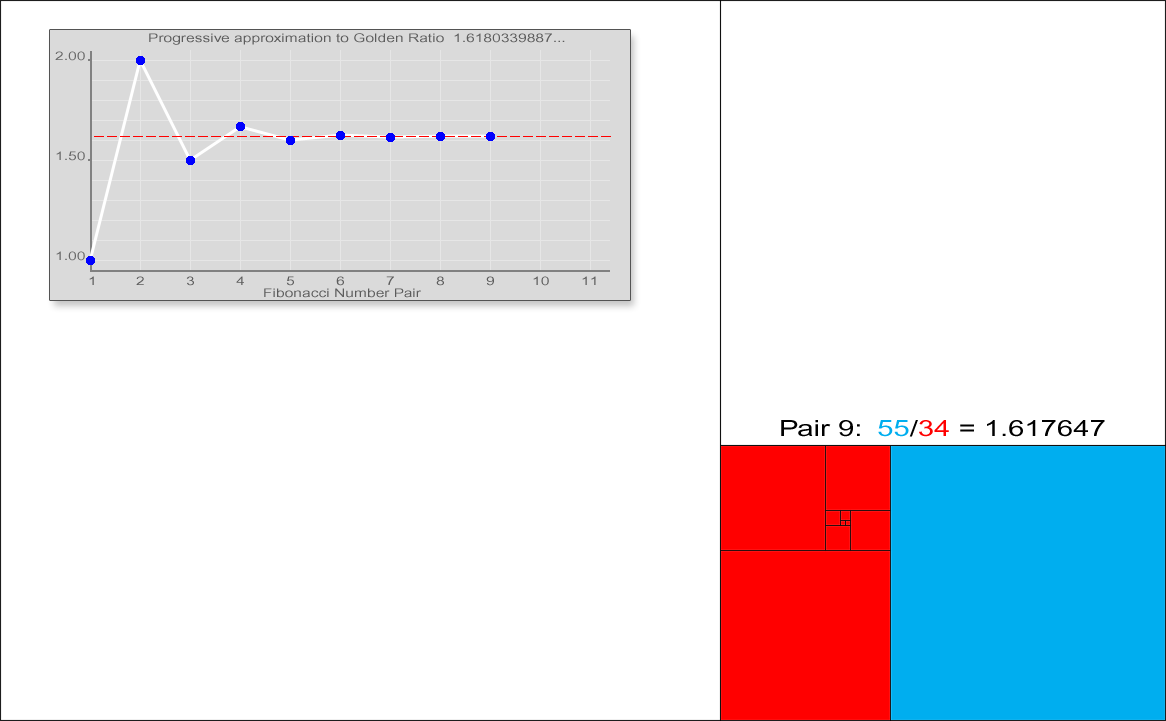
\includegraphics[width=0.9\textwidth]{goldenschnitt/frame_08.png}}
        \only<10>{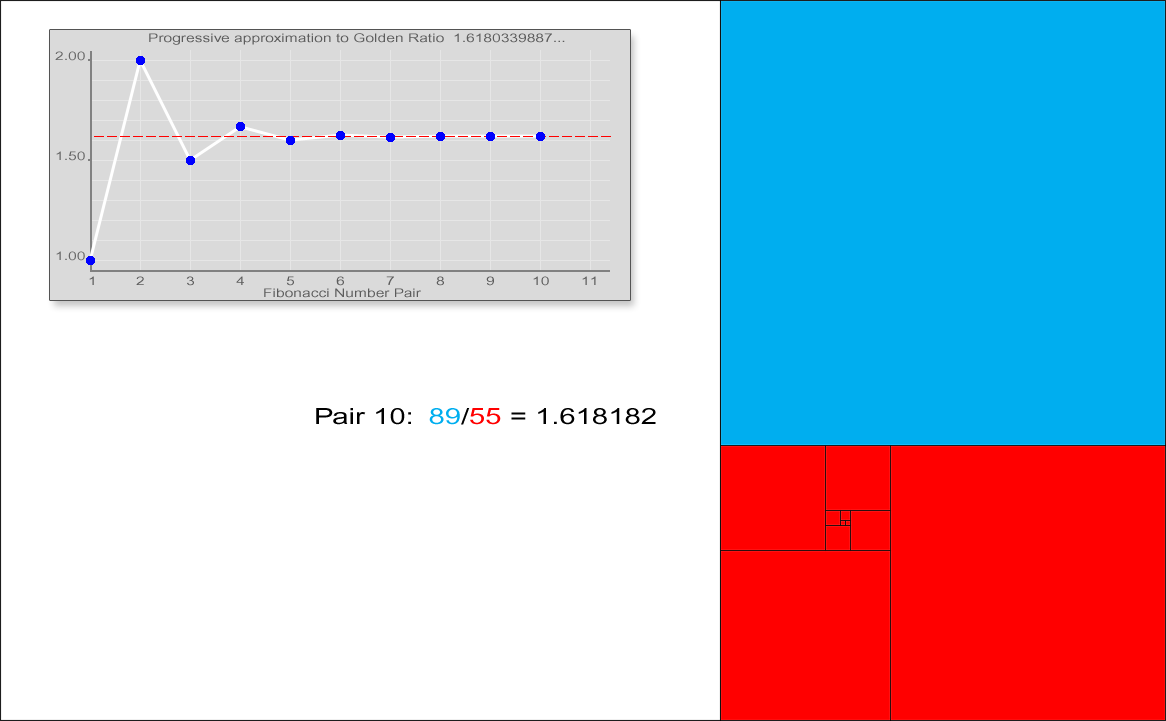
\includegraphics[width=0.9\textwidth]{goldenschnitt/frame_09.png}}
        \only<11>{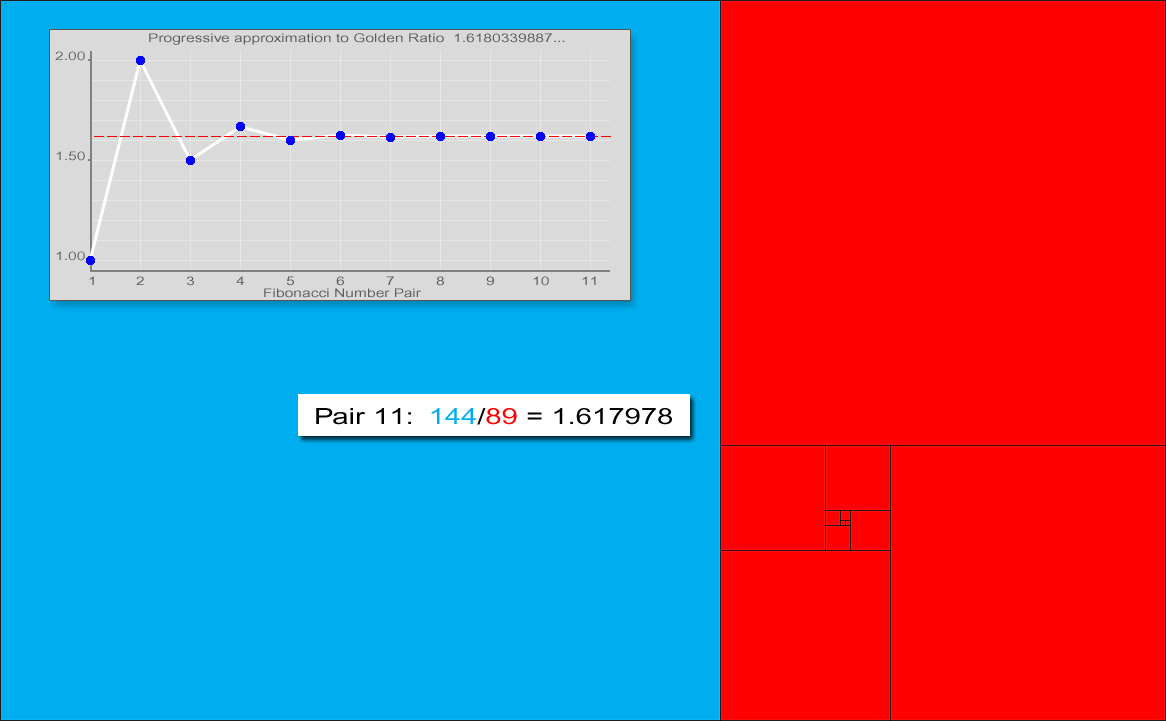
\includegraphics[width=0.9\textwidth]{goldenschnitt/frame_10.png}}
    \end{center}
    
 \vspace{1em}
    \hfill \tiny Quelle: \href{https://en.wikipedia.org/wiki/Fibonacci_sequence#Closed-form_expression}{Wikipedia: FibonacciSequence}
\end{frame} 

\section{Zusatz Aufgaben}

\begin{frame}{Zusatz Aufgaben}
     \subsection{3.8 Rekursiove Formel}
     Finden eine rekursive Formel für die Wahrscheinlichkeit, dass $n$ Personen alle an
verschiedenen Tagen im Jahr Geburtstag haben.  Dabei können wir vereinfachend davon ausgehen,
dass das Jahr 365 Tage hat und die sich die Geburtstage rein zufällig auf die diese 365 Tage
verteilen.  \newline 
\textbf{Ansatz:} $P_{n} = \frac{365}{365} \cdot \frac{364}{365} \cdot \frac{363}{365} \cdot \frac{362}{365} ... \frac{365 - n + 1}{365} $ 

\newline 
\textbf{Allgemein gilt:} $P(n)  = P(n- 1) \cdot \frac{364 - (n -1)}{365}$
\end{frame}


\begin{frame}{3.9 a) Rekursive Formel}
\subsection{3.9}

Rekursive Formel für die Fakultät $n!$:
$n! = 
\begin{cases}
    1 \text{ } \text{ } \text{ } \text{ } \text{ }
    \text{ } \text{ } \text{ } \text{ } \text{ }
    \text{ } \text{ } \text{ } \text{ } \text{ }
    \text{ } \text{ } \text{ }  
    \text{ ,Wenn } n = 0 \\
    n \times (n -1)! \text{ ,Wenn } n > 0
\end{cases}
\end{frame}

\begin{frame}{3.9 a) Code zur Formel }
\begin{figure}
    \begin{center}
    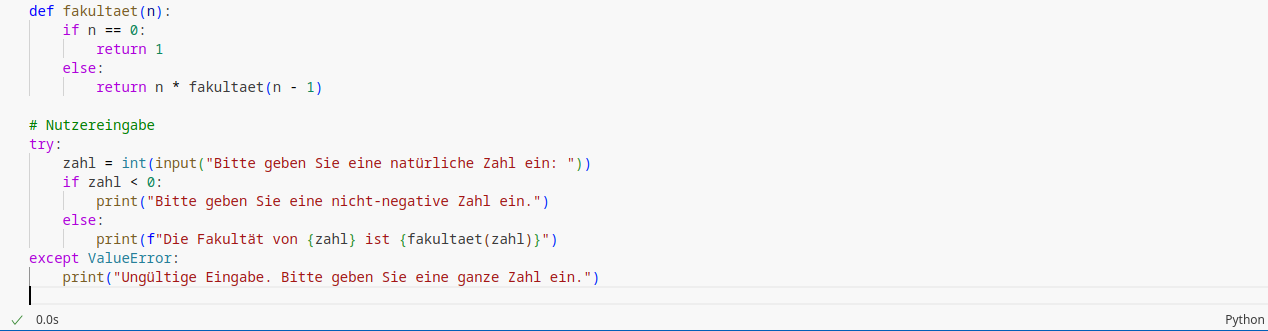
\includegraphics[width=1.8\textwidth]{code/aufg3.9a.png}
    \end{center}
\end{figure}
\end{frame}

\begin{frame}
Rekursive Formel für den Binomialkoeffizienten 
$ \binom{n}{k} $:
$\binom{n}{k} = \begin{cases}
    1     \text{ } \text{ } \text{ } \text{ } \text{ }
    \text{ } \text{ } \text{ } \text{ } \text{ } 
    \text{ } \text{ } \text{ } \text{ } \text{ } 
    \text{ } \text{ } \text{ } \text{ } \text{ } 
    \text{,Wenn } k = 0 \text{ oder } k = n \\
    0     \text{ } \text{ } \text{ } \text{ } \text{ }
    \text{ } \text{ } \text{ } \text{ } \text{ } 
    \text{ } \text{ } \text{ } \text{ } \text{ } 
    \text{ } \text{ } \text{ } \text{ } \text{ }  
    \text{,Wenn } k > n \\
    \binom{n-1}{k -1} + \binom{n -1}{k}  
    \text{, Andern falls } 
\end{cases}$        
\end{frame}

\begin{frame}{3.9 b) Code Rekursive Formel }
\begin{figure}
    \begin{center}
        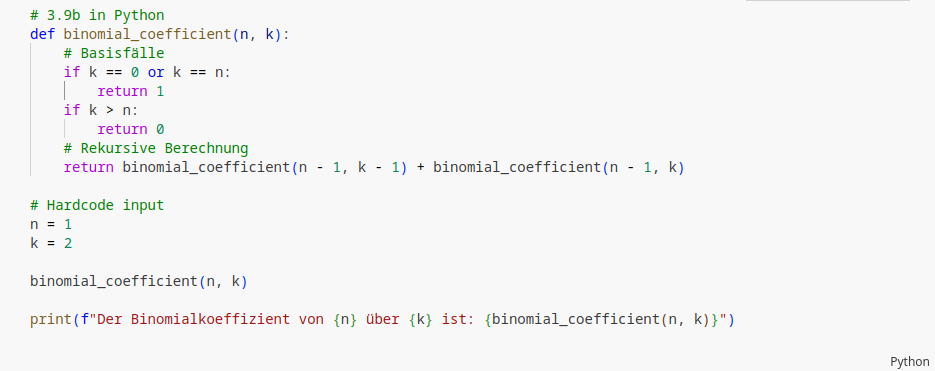
\includegraphics[width=1.3\textwidth]{code/aufg3.9.png}
    \end{center}

\end{figure}


\end{frame}

\begin{frame}{Aufgabe 3.10}
betrachtet werden die folgende rekursiv definierte Folge:
$$b_{n} =
\begin{cases} 
    1, \text{für  } n = 1 \\
    \sqrt{1 + b_{n-1}}, \text{für  } n > 2

\end{cases}$$
Beweisen dass diese Folge gegen den goldenen Schnitt konvergiert:

\[
\lim_{n \to \infty} b_{n}=\frac{1+ \sqrt{5}}{2}
\]
\end{frame}

\begin{frame}
 Um zu zeigen, dass die rekursiv definierte Folge $ b_n $ gegen den goldenen Schnitt $\phi = \frac{1 + \sqrt{5}}{2}$ konvergiert, betrachten wir die Definition der Folge:
$$
b_n = \begin{cases} 
1, & \text{für } n = 1 \\ 
\sqrt{1 + b_{n-1}}, & \text{für } n > 1 
\end{cases}
$$
\end{frame}

\begin{frame}
\textbf{Zu Zeigen, dass die Folge beschränkt und monoton ist:} \\
Zu zeigen, dass die Folge $ b_n$ beschränkt ist.  
\\ Vermutung: $ b_n < \phi $ für alle $ n $. \\
\textbf{Beweis durch Vollständiger Induktion}. 
\textbf{Induktionsanfang:} Für $ n = 1$: $ b_1 = 1 < \phi $. \\
\textbf{Induktionsannahme:} Angenommen, $ b_k < \phi $ für ein $ k \geq 1 .$ \\   
\textbf{Induktionsschritt:} Zeigen, dass $_{k+1} < \phi $:
$$
b_{k+1} = \sqrt{1 + b_k} < \sqrt{1 + \phi}
$$
\end{frame}

\begin{frame}
Da $ \phi = \frac{1 + \sqrt{5}}{2} $, gilt: \\
$
\sqrt{1 + \phi} = \sqrt{1 + \frac{1 + \sqrt{5}}{2}} = \sqrt{\frac{3 + \sqrt{5}}{2}}.
$
Zu zeigen, dass $\sqrt{\frac{3 + \sqrt{5}}{2}} < \phi $: \\

$$
\phi^2 = \left(\frac{1 + \sqrt{5}}{2}\right)^2 = \frac{1 + 2\sqrt{5} + 5}{4} = \frac{6 + 2\sqrt{5}}{4} = \frac{3 + \sqrt{5}}{2}.
$$ \\

Somit ist $ \sqrt{1 + \phi} < \phi \Rightarrow b_{k+1} < \phi $. \\

Durch Induktion folgt, dass $ b_n < \phi $ für alle $ n $. \\
\end{frame}

\begin{frame}
    Zu Zeigen, dass die Folge $ b_n $ monoton wachsend ist, d.h. $ b_n < b_{n+1} \forall n $. \\ 
    \textbf{Zeigen vollständige Induktion:}
    \textbf{Induktionsanfang:} Für $n = 1$ haben wir $ b_1 = 1 < b_2 = \sqrt{1 + 1} = \sqrt{2} .$ \\

\textbf{Induktionsannahme:} Angenommen, $ b_k < b_{k+1} $ \\

\textbf{Induktionsschritt:} Wir zeigen, dass $b_{k+1} < b_{k+2} :$ \\ 
$$
b_{k+2} = \sqrt{1 + b_{k+1}}
$$    
\end{frame}

\begin{frame}
    Da $ b_k < b_{k+1} $, gilt $ 1 + b_k < 1 + b_{k+1} .$  \\
    Da die Funktion $(x) = \sqrt{1 + x}$ monoton wachsend ist, folgt:  \\
$$
b_{k+1} = \sqrt{1 + b_k} < \sqrt{1 + b_{k+1}} = b_{k+2}
$$ \\
    Somit ist $ b_n $ monoton wachsend.
\end{frame}

\begin{frame}
Da $b_n$ eine monoton wachsende und beschränkte Folge ist, konvergiert sie.  \\

Sei $L = \lim_{n \to \infty} b_n $ dann gilt: \\
$$
L = \sqrt{1 + L} => L^2 = 1 + L \implies L^2 - L - 1 = 0 
$$ \\
$$
=> L = \frac{1 \pm \sqrt{5}}{2}
$$

\end{frame}

\begin{frame}
Da $ b_n >= 0$ %positiv ist, nehmen wir die positive Lösung \\
   $$
=> L = \frac{1 + \sqrt{5}}{2} = \phi 
$$  \\
$$
=> \lim_{n \to \infty} b_n = \frac{1 + \sqrt{5}}{2}
$$

\end{frame}

\begin{frame}{Aufgabe 3.11}
    Die folgende rekursiv definierte Folge wird betrachtet:
    \[
    c_n = 
    \begin{cases}
        1, & \text{für } n = 1 \\
        1 + \frac{1}{c_{n-1}}, & \text{für } n > 2
    \end{cases}
    \]
    \bigskip
    Beweisen, dass diese Folge gegen den goldenen Schnitt konvergiert:
    \[
    \lim_{n \to \infty} c_n = \frac{1 + \sqrt{5}}{2}
    \]
\end{frame}


\section{Fazit}
\begin{frame}{Fazit}
        \begin{itemize}
           \item Angewandte Mathematik angenähert 
           \item Anwendung von Rekursion in der Programmierung %(Besonders in funktionalen Paradigma)
           \item Annäherung an der Praxis 
           \item Natur vorkommend 
        \end{itemize}

\end{frame}

\section*{Dankesaussage und Quellen}
\begin{frame}{Danke für das Zuhören}
%Foto: \href{https://momath.org/home/fibonacci-numbers-of-sunflower-seed-spirals/}%{https://momath.org/home/fibonacci-numbers-of-sunflower-seed-spirals/}
Quellen: \url{https://github.com/SpiXFamily/Rekursion-MLL/tree/main/handout/quellen}
\centering
%\href{https://github.com/SpiXFamily/Rekursion-MLL/tree/main/handout/quellen}{Weitere Quellen}
\begin{figure}[H]
    \newline
    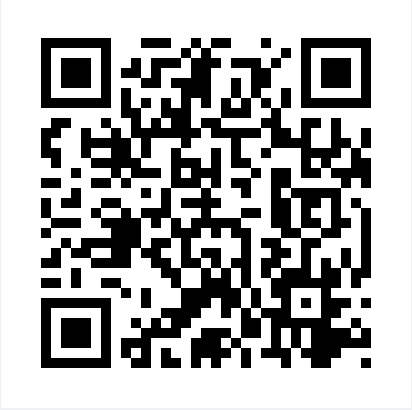
\includegraphics[width=0.5 \textwidth]{bilder/github-qr.png}
    %\caption{\small Quellen https://github.com/SpiXFamily/Rekursion-MLL/tree/main/handout/quellen}
    %\label{https://github.com/SpiXFamily/Rekursion-MLL/tree/main/handout/quellen}
\end{figure}
\end{frame}



\end{document} 
